%% File encoding: UTF-8
%% äöüÄÖÜß  <-- keine deutschen Umlaute hier? UTF-faehigen Editor verwenden!

\documentclass[bachelor,german]{hgbthesis}
\usepackage{dirtree}
% Zulässige Class Options: 
%   Typ der Arbeit: diplom, master (default), bachelor, praktikum 
%   Hauptsprache: german (default), english
%%------------------------------------------------------------
\RequirePackage[utf8]{inputenc}		% remove when using lualatex oder xelatex!
\graphicspath{{images/}}    % name of directory containing the images
\logofile{logo}							% name of logo-PDF in images/ (or use \logofile{} for no logo)
\AddBibFile{literatur}  	% name of the BibTeX (.bib) file


%%%----------------------------------------------------------
\begin{document}
%%%----------------------------------------------------------

% Einträge für ALLE Arbeiten: --------------------------------
\title{Vorlagenmanagement für \emph{Mail}-Service}
\author{Ing. Thomas Herzog}
\studiengang{Software Engineering}
\studienort{Hagenberg}
\abgabedatum{2015}{07}{14}	% {YYYY}{MM}{DD}

%%% zusätzlich für eine Bachelorarbeit: ---------------------
\nummer{S1310307011-A}   % XX...X = Stud-ID, z.B. 0310238045-A  
                        % (A = 1. Bachelorarbeit)
%\semester{Sommersemester 2015} 
%\gegenstand{Einführung in die Tiefere Problematik 1} 
\betreuer{FH-Prof. DI Dr. Dobler} % oder \betreuerin{..}

%%% zusätzlich für einen Praktikumsbericht: -----------------
%\nummer{XXXXXXXXXX-B}   % XX...X = Stud-ID, z.B. 0310238045-B  
                        % (B = 2. Bachelorarbeit)
%\betreuer{Mag.~Pjotr I.~Czar\\Creative Director}  % \betreuerin{..}
\firma{%
   curecomp Software Services GmbH\\
   4020 Linz, Neue Werft, Industriezeile 35
}
\firmenTel{+43 (732) 9015-5565}
\firmenUrl{www.curecomp.com}

%\strictlicense  % erzeugt restriktive Lizenzformel

%%%----------------------------------------------------------
\frontmatter
\maketitle
\tableofcontents
%%%----------------------------------------------------------

\chapter{Kurzfassung}
Die vorliegende Bachelorarbeit behandelt das Vorlagenmanagement für die Anwendung \emph{CleverMail}, die in der theoretischen Bachelorarbeit konzipiert wurde und eine Anwendung ist, die zum Versand von \emph{E-Mails} verwendet wird. Mit dem Vorlagenmanagement können Vorlagen für die \emph{E-Mail}-Nachrichten zur Laufzeit und in mehreren Sprachen verwaltet werden.
\newline
\newline
Das Vorlagenmanagement verwendet mehrere Technologien und Sprachen wie \emph{CDI}, \emph{JSF} und \emph{TypeScript}. Vor allem die Implementierung in Java 8 und die Möglichkeit der Verwendung der neuen sprachspezifischen Funktionalitäten wie \emph{Lambda}-Ausdrücke, Methodenreferenzen und die \emph{Stream-API} haben den Quelltext vereinfacht.
\newline
\newline
Die Integration des Vorlagenmanagements in eine \emph{CDI}-Umgebung war einfach zu realisieren und hat gezeigt, dass ein Softwaremodul in eine \emph{CDI}-Umgebung einfach integriert werden kann, sofern es die nötigen Voraussetzungen erfüllt. Die implementierte \emph{CDI}-Erweiterung wird einfach zu erweitern sein und man könnte mehr Funktionalitäten, die in \emph{CDI} zur Verfügung stehen, verwenden. Es könnten z.B. Erzeuger für Variablen registriert werden, die zur Laufzeit dynamisch Variablen erzeugen, anstatt die Variablen nur beim Start der \emph{CDI}-Umgebung zu registrieren, welche dann über die Lebensdauer der \emph{CDI}-Umgebung  unveränderlich sind. 
\newline
\newline
Während der Entwicklung des Vorlagenmanagements sind keine erwähnenswerten Probleme aufgetreten, alle Funktionalitäten und die Integration konnten einfach implementiert und getestet werden, wobei besonders die Einfachheit der Tests in einer \emph{CDI}-Umgebung hervorgehoben werden muss, die mit der verwendeten Bibliothek \emph{DeltaSpike} einfach aufgesetzt werden können und innerhalb einer Entwicklungsumgebung, ohne Anwendungsserver, lauffähig sind.
\newline
\newline
Die Implementierung des \emph{CKEditor-Plugins} gestaltete sich einfach, da dieser \emph{Editor} gut dokumentiert ist und es bereits Typinformationen für \emph{TypeScript} gibt. Der \emph{Editor TinyMCE}, für den anfangs das \emph{Plugin} entwickelt werden sollte, ist hingegen schlecht dokumentiert, daher wurde auf den \emph{Editor CKEditor} gewechselt. Die Implementierung in \emph{TypeScript} war die richtige Entscheidung, denn es hat die Entwicklung vereinfacht, und der Quelltext ist lesbarer als der Quelltext in \emph{JavaScript}. Für die Zukunft wird \emph{TypeScript} weitere sprachspezifische Möglichkeiten bieten, die den Quelltext noch mehr vereinfachen werden, obwohl eine Migration auf eine neuere Version von \emph{TypeScript} zur Zeit nicht nötig ist.		
\chapter{Abstract}

TODO: Add english summary here
			

%%%----------------------------------------------------------
\mainmatter         % Hauptteil (ab hier arab. Seitenzahlen)
%%%----------------------------------------------------------

\chapter{Einleitung}
\label{cha:Einleitung}
Die vorliegende Sachlage beschäftigt sich mit der Konzeption und Implementierung eines Vorlagen-\emph{Management} für den in der theoretischen Bachelorarbeit konzipierten \emph{Mail}-Service. Das Vorlagen-\emph{Management} stellt einen essentiellen Teil des \emph{Mail}-Service dar, mit dem sich parametrisierte \emph{E-Mail}-Vorlagen erstellen lassen. Das Vorlagen-\emph{Management} soll es den BenutzerInnen ermöglichen einfach eigene parametrisierte \emph{E-Mail}-Vorlagen zu erstellen, die in einer Anwendung, die den \emph{Mail}-Service nutzen, verwendet werden können, um benutzerspezifische \emph{E-Mail}-Nachrichten zu versenden. Mit dem Vorlagen-\emph{Management} ist es nicht mehr erforderlich die \emph{E-Mail}-Vorlagen statisch zu definieren und die \emph{E-Mail}-Vorlagen können von den Benutzerinnen nach ihren Wünschen angepasst werden.  

\section{Das Unternehmen curecomp Software Service GmbH}
Diese Arbeit wird in Zusammenarbeit mit dem Unternehmen \emph{curecomp Software Service GembH} erstellt. Das Unternehmen \emph{curecomp} ist ein ein Dienstleister im \emph{Supplier-Relationship-Management (SRM)} und betreibt eine eigene Softwarelösung namens \emph{clevercure}. Die Softwarelösung \emph{clevercure} besteht aus den folgenden Anwendungen:
\begin{itemize}
	\item\emph{CleverWeb} ist eine \emph{Web}-Anwendung für den webbasierten Zugriff auf \emph{clevercure}.
	\item\emph{CleverInterface} ist eine Schnittstellen-Anwendung für den XML-basierten Datenimport /-export zwischen clevercure und den ERP-Systemen der Kunden.
	\item\emph{CleverSupport} ist eine unternehmensinterne \emph{Web}-Anwendung für die Abwicklung von \emph{Support}-Prozessen.
	\item\emph{CleverDocument} ist ein Dokumentenmanagementsystem für die Verwaltung aller anfallender Dokumente innerhalb von \emph{clevercure}.
	\item\emph{CCMail} ist die bestehende \emph{Mail}-Anwendung für den Versand aller innerhalb \emph{clevercure} anfallender \emph{E-Mail}-Nachrichten.
\end{itemize}
\ \newline
Wie bereits in der theoretischen Bachelorarbeit behandelt, wird \emph{CCMail} von \emph{CleverMail} abgelöst werden, wobei dass in dieser Arbeit behandelte Vorlagenmanagement die Grundlage für \emph{CleverMail} darstellt. Alle Anwendung innerhalb der Softwarelösung \emph{clevercure} haben die Anforderung das \emph{E-Mail}-Vorlagen parametrisiert und benutzerdefiniert erstellt werden können. Diese Anforderung wird mit dem Vorlagenmanagement erfüllt.

\section{Das Vorlagenmanagement für den \emph{Mail}-Service}
Mit dem Vorlagenmanagement können \emph{E-Mail}-Vorlagen einerseits von den EntwicklerInnen und BenutzerInnen benutzerdefiniert und parametrisiert erstellt werden. Damit können \emph{E-Mail}-Vorlagen dynamisch auch zur Laufzeit erstellt, modifiziert und gelöscht werden. Es sind keine statischen \emph{E-Mail}-Vorlagen mehr nötig und alle damit verbunden Nachteile wie z.B. 
\begin{itemize}
	\item das neu Kompilieren und Einspielen bei Änderungen der \emph{E-Mail}-Vorlagen,
	\item keine Möglichkeit für benutzerdefinierten Vorlagen oder
	\item keine Möglichkeit der Nutzung von dynamischen Parametern in den \emph{E-Mail}-Vorlagen
\end{itemize}
\ \newline
eliminiert werden. Das Vorlagenmanagement kann auch in einem anderen Kontext verwendet werden, wobei diese Arbeit sich  ausschließlich mit der Verwendung des Vorlagenmanagement innerhalb des \emph{Mail}-Service beschäftigen wird. 
\newline
TODO: Add graphic about template management
\newline

\section{Die Rahmenbedingungen}
Das Vorlagenmanagement wird in Java in der Version 8 implementiert und wird sich an der \emph{Java-Enterprise-Edition 7 (JEE-7)} Spezifikation orientieren, wobei folgende Teilspezifikationen Anwendung finden.
\begin{itemize}
	\item \emph{JPA 2.1} ist die Spezifikation für die Persistenz.
	\item \emph{CDI 1.1} ist die Spezifikation für kontextabhängige Injektion innerhalb einer \emph{JEE7}-Umgebung.
	\item \emph{JSF 2.2} ist die Spezifikation der \emph{View}-Technologie. 
\end{itemize}
\ \newline
Damit wird das Vorlagenmanagement mit den aktuellsten Standards implementiert und wird daher für die Zukunft gut gewappnet sein. Die Funktionalität des Vorlagenmanagement wird weitestgehend ohne die Verwendung spezieller Bibliotheken implementiert, wobei folgende Integrationen zur Verfügung gestellt werden.
\begin{itemize}
	\item \emph{CDI}-Integration:
	\newline
	Innerhalb eines \emph{CDI-Containers} werden Objekte kontextabhängig zur Verfügung gestellt.
	\item \emph{JSF}-Integration:
	\newline
	Mit der \emph{View}-Technologie \emph{JSF} wird eine Webseite erstellt, über die die Vorlagen verwaltet werden können.
	\item \emph{Typescript}-Integration:
	\newline
	Mit \emph{Typescript} wird ein \emph{Plugin} für den \emph{Rich-Editor CKEditor} implementiert, welches die Variablen für eine \emph{E-Mail}-Vorlage innerhalb des \emph{CKEditors} verwaltet.
\end{itemize} 
\ \newline
Als Entwicklungsumgebung wird die \emph{IDE Intellij} verwendet, die eine bekannte Entwicklungsumgebung im \emph{Java}-Umfeld darstellt und ein Produkt des Unternehmens \emph{Jetbrains} mit Sitz in Tschechien ist. Als Applikationsserver wird \emph{Wildfly 10.x}, vormals \emph{JbossAS} genannt, des Unternehmens  \emph{Redhat} verwendet, der ein zertifizierter \emph{JEE-7}-Server ist und somit alle benötigten Spezifikationen unterstützt.

\chapter{Das Ziel des Projekts}
\label{cha:Zielsetzung}
Das Ziel des Projekts Vorlagenmanagement für \emph{Mail-Service} ist die Entwicklung der Softwarekomponente Vorlagenmanagement für die Verwendung in \emph{CleverMail}, mit dem Vorlagen verwaltet werden können. Das Vorlagenmanagement stellt einen essentiellen Teil von \emph{CleverMail} dar und wird auch von mehreren Anwendungen innerhalb von \emph{clevercure} verwendet werden. Die verschiedenen Anwendungen, die das Vorlagenmanagement verwenden, sind ebenfalls in Java implementiert, werden aber in unterschiedlichen Laufzeitumgebungen betrieben wie z.B:
\begin{itemize}
	\item Der \emph{IBM-Integration-Bus (IIB)}
	\newline
	ist ein proprietäres Produkt des Unternehmens \emph{IBM}, das für die \emph{XML}-Konvertierungen und den \emph{XML}-basierten Datenimport und Datenexport verwendet wird.
	\item Der Anwendungsserver \emph{Wildfly}
	\newline
	ist ein zertifizierter und frei verfügbarer \emph{JEE-7} Applikationsserver des Unternehmens \emph{Redhat}.
\end{itemize} 
\ \newline
Die verschiedenen Anwendungen von \emph{clevercure} müssen mit möglichst wenig Aufwand in der Lage sein, Vorlagen zu verwenden und \emph{E-Mail}-Nachrichten auf Basis dieser Vorlagen zu erstellen. Dabei müssen die Abhängigkeiten der Anwendungen zum Vorlagenmanagement so gering wie möglich gehalten werden, sowie nur vorgegebene Schnittstellen verwendet werden dürfen. Wird eine \emph{E-Mail}-Nachricht von einer Anwendung auf Basis einer Vorlage erstellt, so müssen die  aktuellen Werte der enthaltenen Variablen der Vorlage beim Zeitpunkt des Erstellens der \emph{E-Mail}-Nachricht ermittelt und serialisiert werden, damit die \emph{E-Mail}-Nachricht mit dem selben Inhalt erneut versendet werden kann. Für die Anwendungen darf nicht erkennbar sein, wie die \emph{E-Mail}-Nachrichten nach ihrer Erstellung weiter verwendet werden. Zurzeit interagieren die Anwendungen direkt mit der Datenbank, anstatt von ihr abstrahiert zu sein und sind daher stark an die bestehende Anwendung \emph{CCMail} gekoppelt bzw. an das Datenbankmodell der Anwendung \emph{CCMail}.
\newpage

\section{Die funktionalen Ziele}
Für das Vorlagenmanagement wurden die folgende funktionalen Anforderungen definiert, die umgesetzt werden müssen.

\subsection{Die Variablen für die Vorlagen}
Die Vorlagen werden für einen bestimmten \emph{Mail}-Typ definiert, der in einen bestimmten Kontext verwendet wird wie z.B.
\begin{itemize}
	\item ein BenutzerIn wurde erstellt,
	\item eine Bestellung wurde erstellt oder
	\item ein Dokument wurde hochgeladen.
\end{itemize}
\ \newline
Für die Vorlagen, die für einen bestimmten \emph{Mail}-Typ erstellt werden, müssen Variablen zur Verfügung gestellt werden können wie z.B.:
\begin{itemize}
	\item Die Variable \emph{CURRENT\_USER}
	\newline
	ist der Benutzer, der die \emph{E-Mail}-Nachricht erstellt halt.
	\item Die Variable \emph{ORDER\_NUMBER}
	\newline
	ist die Nummer der erstellten Bestellung.
\end{itemize}
\ \newline
Die EntwicklerInnen müssen für einen bestimmten \emph{Mail}-Typ in der Lage sein einfach Variablen zu definieren, die von den BenutzerInnen, beim Erstellen einer Vorlage für den korrespondierenden \emph{Mail-Typ}, frei verwendet werden können. Die Variablen müssen auch global definiert werden und prinzipiell in allen Vorlagen verwendbar sein. Die EntwicklerInnen müssen in der Lage sein die Menge der zur Verfügung stehenden Variablen zur Laufzeit aufgrund von bestimmten Zuständen verändern zu können. Die Menge der Variablen könnte z.B. von Berechtigungen der BenutzerInnen abhängig sein.

\subsection{Die Mehrsprachigkeit der Variablen}
Die zur Verfügung stehenden Variablen werden durch die EntwicklerInnen statisch definiert und müssen einen Bezeichnung und eine Beschreibung zur Verfügung stellen. Die Bezeichnung und die Beschreibung der Variable müssen mehrsprachig zur Verfügung stehen, wobei als Standardsprache Englisch zu verwenden ist. Die Mehrsprachigkeit soll über \emph{Java-Properties}-Dateien abgebildet werden, wobei als Zeichenkodierung \emph{UTF8} zu verwenden ist, obwohl \emph{Java- Properties}-Dateien laut Spezifikation die Zeichenkodierung \emph{ISO 8859-1} verwenden müssen.

\subsection{Die automatische Registrierung der Variablen}
Innerhalb einer \emph{CDI}-Umgebung sollen die definierten Variablen beim Start der \emph{CDI}-Umgebung automatisch gefunden und registriert werden. Die automatische Registrierung der Variablen muss mit einer \emph{CDI}-Erweiterung realisiert werden, die beim Start der \emph{CDI}-Umgebung die Variablen findet, registriert und über die Anwendungslebensdauer persistent hält. Mit einer automatischen Registrierung der Variablen wird erreicht, dass neu definierte Variablen automatisch gefunden und registriert werden und somit nicht manuell registriert werden müssen. Ein manuelles Registrieren der Variablen birgt das Risiko in sich, dass Variablen vergessen werden könnten registriert zu werden.

\subsection{Die Mehrsprachigkeit der Vorlagen}
Die Vorlagen müssen in mehreren Sprachen erstellt und verwaltet werden können, wobei eine Sprache als Standardsprache zu definieren ist und es für diese Sprache immer einen Eintrag geben muss. Auf die Standardsprache wird zurückgegriffen, wenn es für eine angeforderte Sprache keinen Eintrag gibt. Somit ist gewährleistet, dass für jede angeforderte Sprache immer eine Vorlage zur Verfügung steht. Es ist nicht erforderlich dass die Menge und Position der Variablen in einer Vorlage über alle definierte Sprachen gleich sind. Es dürfen in einer Vorlage, die in mehreren Sprachen definiert wurde, eine unterschiedliche Anzahl von Variablen, unterschiedliche Variablen  und unterschiedliche Positionen der Variablen definiert sein.

\subsection{Die Persistenz der Vorlagen}
\label{sec:sub-template-variable-persistenz}
Die Vorlagen müssen innerhalb einer Datenbank persistent gehalten werden. Da das Vorlagenmanagement vorerst exklusiv für \emph{CleverMail} verwendet wird, muss die Persistenz der Vorlagen innerhalb des \emph{Mail}-DB-Schema von \emph{CleverMail} realisiert werden. Die persistenten Vorlagen müssen versionierbar sein, damit diese von anderen Entitäten referenziert werden können, ohne dass die Gefahr besteht, dass die referenzierte Vorlage verändert wurde.    Die Versionierung soll die Konsistenz der Vorlagen sicherstellen, sodass serialisierte Daten für eine Vorlage konsistent mit den enthaltenen Variablen der Vorlage sind. Vorlagen müssen explizit freigegeben werden, bevor diese verwendet dürfen. Nach einer Freigabe darf die Vorlage nicht mehr geändert werden.

\subsection{Die Verwaltung der Vorlagen über eine Webseite}
\label{sec:sub-template-management-website}
Die Vorlagen müssen über eine Webseite verwaltet werden können. Die Webseite muss mit der \emph{View}-Technologie \emph{JSF} implementiert werden. Über einen \emph{FacesConverter} soll die Vorlage von ihrer \emph{HTML}-Repräsentation in die Repräsentation der verwendeten \emph{Template-Engine} konvertiert werden und visa versa. Der Quelltext aus Abbildung \ref{prog:html-markup-vorlage} zeigt ein \emph{HTML-Markup} einer Vorlage, wie es in der Webseite  bzw. innerhalb des \emph{Editors CKEditor} verwendet wird. Die Variablen werden als \emph{HTML-Tags} repräsentiert, aus denen die Variable wieder hergestellt werden kann.
\begin{program}[h]
	\caption{Beispiel eines \emph{HTML-Markup} einer Vorlage}
	\label{prog:html-markup-vorlage}
	\begin{HtmlCode}[numbers=none]
	<p>Das ist eine Variable:</p>
	<p>
		<span class="variable" 
		      title="Die Beschreibung der Variable" 
		      data-variable="VAR_ID">
   			Die Bezeichnung der Variable
		</span>
	</p>
	\end{HtmlCode}
\end{program}
\ \newline
Der Quelltext aus Abbildung \ref{prog:freemarker-markup-vorlage} zeigt das konvertierte \emph{HTML-Markup} aus Abbildung \ref{prog:html-markup-vorlage} als \emph{Freemarker}-Vorlage .
\begin{program}[h]
	\caption{Konvertiertes \emph{HTML-Markup} als \emph{Freemarker-Template}}
	\label{prog:freemarker-markup-vorlage}
	\begin{GenericCode}[numbers=none]
	<p>Das ist eine Variable:</p>
	<p>
		${module.core.VariableHolder["VAR_ID"]!("Nicht verfügbar")}
	</p>	
	\end{GenericCode}
\end{program}
\ \newline
Auf der Webseite muss der \emph{JavaScript} basierte \emph{Editor CKEditor} verwendet werden, weil für diesen \emph{Editor} von \emph{PrimeFaces-Extensions} eine \emph{JSF}-Integartion, in Form einer \emph{JSF}-Komponente, zur Verfügung gestellt wird. Es muss der \emph{Editor CKEditor} verwendet werden, weil eine Integration in den Lebenszyklus von \emph{JSF} notwendig ist, damit z.B. auf \emph{AJAX-Reqeust} reagiert werden kann, wie es in \emph{JSF} üblich ist.

\section{Die technischen Ziele}
\label{sec:technical-goals}
Es wurden die folgenden technischen Zile definiert.
\begin{itemize}
	\item Die Entwicklung in \emph{Java 8},
	\item die Entwicklung mit der Plattform \emph{JEE-7},
	\item die Integration in eine \emph{CDI}-Umgebung,
	\item die Integration in \emph{JSF} und
	\item die Entwicklung als eigene Softwarekomponente.
\end{itemize}
Das Vorlagenmanagement muss Schnittstellen definieren, die die Funktionalitäten des Vorlagenmanagements nach außen offenlegen, ohne dass die Anwendungen in Berüghrung mit den konkreten Implementierungen kommen.
\chapter{Das Lösungskonzept}
\label{cha:Lösungskonzept}
In diesem Kapitel wird der Lösungsansatz und die Spezifikation des Vorlagenmanagements erörtert. Bei der Spezifikation handelt es sich um Schnittstellen und abstrakte Klassen, die die Struktur des Vorlagenmanagements definieren. Diese Schnittstellen und abstrakten erlauben es Implementierungen für verschiedene \emph{Template-Engines} wie z.B
\begin{itemize}
	\item \emph{Freemakrer},
	\item \emph{Velocity} oder
	\item \emph{Thymeleaf}
\end{itemize}
zur Verfügung zu stellen, wobei die abstrakten Klassen die gemeinsam nutzbare Logik implementieren, die über die verschiedenen \emph{Template-Engines} verwendet werden kann.
\newline
\newline
Mit der Möglichkeit die verschiedensten \emph{Template-Engines} verwenden zu können, wird erreicht dass das Vorlagenmanagement sehr flexibel ist. Bei dem Wechsel zu einer anderen \emph{Template-Engine} müssen nur die \emph{Expressions} einer Vorlagen in die \emph{Template-Engine} spezifischen \emph{Expressions} umgewandelt werden.
\ \newpage

\section{Die Spezifikation des Vorlagenmanagements}
Dieses Kapitel behandelt die erstellten Spezifikationen des Vorlagenmanagements. Auf Basis dieser Spezifikationen wird das Vorlagenmanagement und die Integrationen in die verschiedenen Umgebungen und Technologien implementiert. Die erstellte Spezifikationen sind frei von Abhängigkeiten auf konkrete Implementierungen jeglicher Art. Sie haben nur Abhängigkeiten auf andere Spezifikationen wie die \emph{JEE-7} Spezifikation.

\begin{figure}[h]
\centering
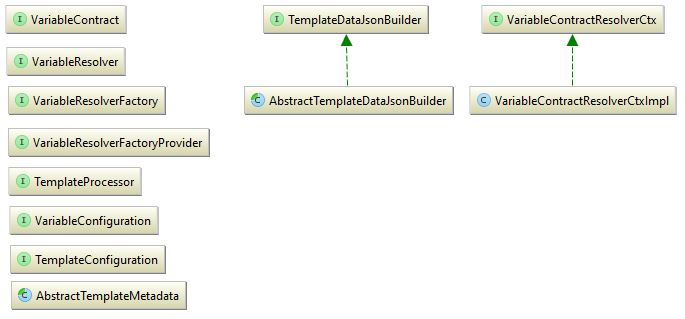
\includegraphics[scale=0.73]{20160710_template-logic-api.jpg} %{CS0031}
\caption{Klassenhierarchie der Vorlagen-\emph{API}}
\label{fig:template-logic-api-hierarchy}
\end{figure}

\subsection{Die Schnittstellen und abstrakten Klassen}
Dieser Abschnitt behandelt die implementierten Schnittstellen und abstrakten Klassen des Vorlagenmanagements. Die abstrakten Klassen implementieren die gemeinsam nutzbaren Funktionalitäten, welche von alle konkreten Implementierungen des Vorlagenmanagements genutzt werden können. Diese Spezifikationen spezifizieren Aspekte des Vorlagenmanagements wie
\begin{enumerate}
	\item das Variablenmanagement innerhalb des Vorlagenmanagement,
	\item die Handhabung von Variablen in einer Vorlage 
	\item die Abbildung der Metadaten einer Voralge und 
	\item das Erstellen des \emph{JSON}-Objekts, welches die Daten für die Vorlage beinhaltet.
\end{enumerate}

\subsubsection{Die Schnittstelle \emph{VariableContract}}
\label{sec:variableContract}
Die Schnittstelle \emph{VariableContract} spezifiziert eine Variable, die in einer Vorlage verwendet werden kann. Objekte dieser Schnittstelle werden beim Anwendungsstart registriert und können grundsätzlich in allen Vorlagen verwendet werden. Eine Variable ist einem Modul zugeordnet, in dem die Variable bezüglich ihres Namen eindeutig sein muss. Das Modul wird über einen \emph{String} definiert. Die Mehrsprachigkeit einer Variable wird über Enumerationen realisiert, wobei jede Variable jeweils einen Schlüssel für den Titel und die Beschreibung bereit stellt. 
\newline
\newline
Da es sich bei einer Variable um statische Daten handelt, also die Variablen sind schon zur Kompilierungszeit bekannt, ist angedacht, dass die Variablen mit dem \emph{Java}-Typ \emph{enum} implementiert werden, dass die Schnittstelle \emph{VariableContract} implementiert. Durch die Abbildung der Variablen mit dem \emph{Java}-Typ \emph{enum} können mehrere Variablen in einer Klasse definiert werden, wobei eine einzelne Enumeration ein Objekt der Schnittstelle \emph{VariableContract} darstellt. Alle Variablen die mit einer \emph{enum} abgebildet werden, sollten demselben Modul zugeordnet sein, obwohl dies nicht zwingend erforderlich ist. Die Zuordnung der Variablen zum selben Modul erleichtert die Wartung und Strukturierung der Variablen. Die Variablen, die mit einer \emph{enum} definiert wurden, werden innerhalb des Vorlagenmanagements trotzdem als einzelne Objekte der Schnittstelle \emph{VariableContract} betrachtet. Die Tatsache dass die Variablen mit einer \emph{enum} abgebildet wurden, ist für das Vorlagenmanagement nur beim Registrieren der Variablen von belang und nicht bei deren weiterer Verwendung.
\newline
\newline
Eine Variable ist über seine \emph{Id} eindeutig referenzierbar, wobei sich die \emph{Id} aus dem Modulnamen und den Variablennamen zusammensetzt (Bsp. module.core.VAR\_1). Die \emph{Id} hält sich dabei an die Namenskonvention eines \emph{Java}-Paketnamen. Da der Variablenname immer auf diese Weise zusammengesetzt werden sollte, wurde die Methode \emph{String getId();} als \emph{default Methode} implementiert, was seit \emph{Java 8} möglich ist. Ein EntwicklerIn muss diese Methode nicht mehr implementieren, obwohl es immer noch möglich ist diese Methode zu überschreiben. Auch die Methode \emph{String toInfoString()} wurde als \emph{default Methode} implementiert, da auch diese Methode nicht von den EntwicklerInnen implementiert werden sollte, da ihre Funktionalität sich nicht ändern sollte.
\newpage

\begin{program}[h]
\caption{VariableContract.java}
\label{prog:variableContract}
\begin{JavaCode}
public interface VariableContract extends Serializable {

    String getName();

    String getModule();

    Enum<?> getInfoKey();

    Enum<?> getLabelKey();

    default String getId() {      
        return getModule() + "." + getName();
    }

    default String toInfoString() {
        final String ls = System.lineSeparator();
        final StringBuilder sb = new StringBuilder();
        sb.append("contract  : ").append(this.getClass().getName())
          .append(ls)
          .append("id        : ").append(getId())
          .append(ls)
          .append("name      : ").append(getName())
          .append(ls)
          .append("label-key : ").append((getLabelKey() != null) 
                                          ? getLabelKey().name() 
                                          : "not available")
          .append(ls)
          .append("info-key  : ").append((getInfoKey() != null) 
                                          ? getInfoKey().name() 
                                          : "not available")
          .append(ls)
          .toString();
    }
}
\end{JavaCode}
\end{program}

\subsubsection{Die Schnittstelle \emph{VariableResolver}}
\label{sec:variableResolver}
Die Schnittstelle \emph{VariableResolver} spezifiziert wie der aktuelle Wert der Variablen aufgelöst wird. Eine Variable wird in einer Vorlage verwendet und beim Erstellen eines Datenbankeintrags, der diese Vorlage verwendet, müssen die aktuellen Werte der beinhalteten Variablen aufgelöst werden. Da der aktuelle Wert der Variable kontextabhängig ist, wird beim Auflösen des Werts der Variable ein Kontext bereitgestellt, über den kontextabhängige Daten vom EntwicklerIn bereitgestellt werden können, die in einer Implementierung der Schnittstelle \emph{VariableResolver} angewendet werden können. Dadurch kann die Variable in mehreren Kontexten verwendet werden und auch kontextabhängig aufgelöst werden.
\begin{program}[h]
\caption{VariableResolver.java}
\label{prog:variableResolver}
\begin{JavaCode}
@FunctionalInterface
public interface VariableResolver {

    String resolve(VariableContract variable,
                   VariableContractResolverContext ctx);
}
\end{JavaCode}
\end{program}
\ \newline
Die Schnittstelle \emph{VariableResolver} wurde als \emph{FunctionalInterface} implementiert. Ein \emph{FunctionalInterface} ist eine Schnittstelle, die nur eine abstrakte Methode definiert, die implementiert werden muss. Eine Implementierung eines \emph{FunctionalInterface} kann über eine \emph{Lambda}-Funktion oder Methodenreferenz bereitgestellt werden, wodurch die Notwendigkeit einer anonymen Implementierung oder der Implementierung einer Klasse für diese Schnittstelle entfällt. Dieser Ansatz macht den Quelltext lesbarer, obwohl angemerkt sei, dass dieser Ansatz sich negativ auf das Laufzeitverhalten auswirkt, was in der Art und Weise der Ausführung einer \emph{Lambda}-Funktion oder Methodenreferenz begründet ist. Die negativen Auswirkungen auf das Laufzeitverhalten können, im Bezug auf das Vorlagenmanagement, vernachlässigt werden.

\subsubsection{Die Schnittstelle \emph{VariableResolverFactory}}
\label{sec:variableResolverFactory}
Die Schnittstelle \emph{VariableResolverFactory} spezifiziert wie Objekte der Schnittstelle \emph{VariableResolver} produziert werden. Objekte dieser Schnittstelle können Objekte der Schnittstelle \emph{VariableResolver} für jede Implementierung der Schnittstelle \emph{VariableContract} produzieren, obwohl es zu empfohlen ist, dass es eine Implementierung der Schnittstelle \emph{VariableResolverFactory} je Modul zur Verfügung gestellt wird.

\begin{program}[h]
\caption{VariableResolverFactory.java}
\label{prog:variableResolverFactory}
\begin{JavaCode}
@FunctionalInterface
public interface VariableResolverFactory extends Serializable {

  VariableResolver getVariableResolver(VariableContract contract,
                                       VariableContractResolverCtx ctx);
}
\end{JavaCode}
\end{program}
\ \newline
Die Schnittstelle \emph{VariableResolver} wurde ebenfalls als \emph{FunctionalInterface} implementiert, damit Implementierungen über eine \emph{Lambda}-Funktion oder eine Methodenreferenz bereitgestellt werden kann.

\subsubsection{Die Schnittstelle \emph{VariableResolverFactoryProvider}}
\label{sec:VariableResolverFactoryProvider}
Die Schnittstelle \emph{VariableContractFactoryProvider} spezifiziert wie Objekte der Schnittstelle \emph{VariableResolverFacotry} produziert werden. Ein Objekt der Schnittstelle \emph{VariableResolverFactoryProvider} kann Objekte der Schnittstelle \emph{VariableResolverFactory} für die Schnittstelle \emph{VariableContract}, einer Ableitung von dieser Schnittstelle oder einer konkreten Implementierung dieser Schnittstelle zur Verfügung stellen. 

\begin{program}[h]
\caption{VariableResolverFactoryProvider.java}
\label{prog:variableResolverFactoryProvider}
\begin{JavaCode}
@FunctionalInterface
public interface VariableResolverFactoryProvider extends Serializable {

    VariableResolverFactory getVariableResolverFactory
            (Class<? extends VariableContract> contractType);
}
\end{JavaCode}
\end{program}
\ \newline
Die Schnittstelle \emph{VariableResolverFactoryProvider} wurde auch als \emph{FunctionalInterface} implementiert um Implementierungen über eine \emph{Lambda}-Funktion oder Methodenreferenz zur Verfügung stellen zu können.

\subsubsection{Die Schnittstelle \emph{VariableContractResolverCtx}}
\label{sec:variableResolverFactoryProvider}
Die Schnittstelle \emph{VariableContractResolverCtx} spezifiziert den Kontext, der bei der beim Auflösen des aktuellen Werts einer Variablen zur Verfügung gestellt wird. Dieser Kontext stellt alle Daten bereit, die beim Auflösen des aktuellen Werts einer Variable benötigt werden. Es wird auch ermöglicht, dass Benutzerdaten im Kontext definiert werden können, die bei beim Auflösen des aktuellen Werts einer Variable verwendet werden können. Es wurde bewusst vermieden, dass beim Auflösen eines aktuellen Werts einer Variable bekannt ist, in welcher Vorlage die Variable verwendet wird. Dadurch bleibt die Handhabung der Variablen einer Vorlage entkoppelt von der Vorlage selbst. Dadurch wäre es möglich die Variablen außerhalb vom Vorlagenmanagements zu verwenden.
\newpage

\begin{program}[h]
\caption{VariableContractResolverCtx.java}
\label{prog:variableContractResolverCtx}
\begin{JavaCode}
public interface VariableContractResolverCtx {

    Locale getLocale();

    ZoneId getZoneId();

    TimeZone getTimeZone();

    <T> T getUserData(Object key,
                      Class<T> clazz);
}
\end{JavaCode}
\end{program}

\subsubsection{Die Schnittstelle \emph{TemplateProcessor}}
\label{sec:templateProcessor}
Die Schnittstelle \emph{TemplateProcessor} spezifiziert wie die Vorlagen behandelt werden. Objekte dieser Schnittstelle können Variablen in einer Vorlage, einer bestimmten \emph{Template-Engine} finden und konvertieren. Ein \emph{TemplateProcessor} muss ebenfalls in der Lage sein ungültige Variablen innerhalb einer Vorlage zu finden, wobei eine ungültige Variable eine Variable ist, die nicht registriert ist und somit auch der aktuelle Wert der Variable nicht aufgelöst werden kann.
\newline
\newline
Eine konkrete Implementierung dieser Schnittstelle ist eine Implementierung für eine bestimmte \emph{Template-Engine}, da die in der Vorlage verwendeten \emph{Expressions} spezifisch für die verwendete \emph{Template-Engine} sind. 
\newline
\newline
Besonders sind beiden folgenden Methoden hervorzuheben.
\begin{JavaCode}[numbers=none]
String replaceExpressions(String template,
                          Function<VariableContract, String> converter);

String replaceCustom(String template,
                     Pattern itemPattern,
                     Function<String, String> converter);
\end{JavaCode}
Diese Methoden verwenden als Formalparameter für den benötigte Konverter ein \emph{FunctionalInterface} namens \emph{Function}, welches von der Sprache \emph{Java 8} bereitgestellt wird. Dadurch ist das Spezifizieren einer eigenen Schnittstelle für die Konvertierung nicht mehr nötig. Der Konverter kann über eine \emph{Lambda}-Funktion oder Methodenreferenz bereitgestellt werden. Dadurch ist die Konvertierung der Variablen einer Vorlage abstrahiert von der Implementierung der Schnittstelle \emph{TemplateProcessor}, wodurch die Variablen durch eine beliebige Repräsentation ersetzt werden können und visa versa.
\newpage

\begin{program}[h]
\caption{TemplateProcessor.java}
\label{prog:templateProcessor}
\begin{JavaCode}
public interface TemplateProcessor {

    String replaceExpressions(String template,
                              Function<VariableContract, String> converter);

    String replaceCustom(String template,
                         Pattern itemPattern,
                         Function<String, String> converter);

    Set<VariableContract> resolveExpressions(String template);

    Set<String> resolveInvalidExpressions(String template);

    String variableToExpression(VariableContract contract);

    VariableContract expressionToVariable(String expression);
}
\end{JavaCode}
\end{program}

\subsubsection{Die Schnittstelle \emph{TemplateDataJsonBuilder}}
\label{sec:templateDataJsonBuilder}
Die Schnittstelle \emph{TemplateDataJsonBuilder} spezifiziert die Signatur eines \emph{Builders}, der das \emph{JSON}-Objekt erstellt, welches die Daten für das Parsen einer Vorlage enthält. Eine Anforderung ist es, die \emph{E-Mail}-Nachrichten persistent zu halten, wobei nach der Erstellung einer \emph{E-Mail}-Nachricht, dessen Inhalt unveränderbar sein soll. Es werden die Metadaten wie die Sprache sowie die aufgelösten Werte der in der Vorlage enthaltenen Variablen mit einem \emph{JSON}-Objekt persistent gehalten. Es könnte auch die Vorlage geparst werden und die gesamte geparste Vorlage persistent gehalten werden, wodurch aber die Menge an persistent gehaltenen Daten stark ansteigen würde. Da nur die Metadaten und die Werte der Variablen persistent gehalten werden, wird die Menge an persistent gehaltenen Daten so klein wie möglich gehalten, da nur die variablen Teile einer Vorlage für eine \emph{E-Mail}-Nachricht persistent gehalten werden. Mit diesem \emph{JSON}-Objekt kann die korrespondierende Vorlage zu jedem Zeitpunkt mit demselben Resultat erneut geparst werden.
\newline
\newline
Es wurde hier das \emph{Builder}-Muster angewendet, da sich die Konfiguration des \emph{Builders} mit einer \emph{Fluent-API}, wie bei einem \emph{Builder} üblich, sehr gut abbilden lässt. Die Schnittstelle \emph{TemplateDataJsonBuilder} spezifiziert folgende Terminalmethoden.
\begin{itemize}
	\item\emph{TemplateRequestJson toJsonModel()} ist die Methode, die das \emph{JSON}-Objekt in Form eines \emph{Java}-Objekts zurückliefert.
	\item\emph{String toJsonString()} ist die Methode, die das \emph{JSON}-Objekt als String zurückliefert.
	\item\emph{Map<String, Object> toJsonMap()} ist die Methode, die das \emph{JSON}-Objekt in Form einer \emph{java.util.Map} zurückliefert.
\end{itemize}  
Folgender Quelltext illustriert, wie der \emph{Builder} verwendet wird.
\begin{JavaCode}[numbers=none]
builder.withStrictMode() 
       .withLocalization(localeObj, zoneIdObj)
       .withTemplate(templateMetadataObj)
       .withUserData(userDataMap)
       .withVariableResolverFactoryProvider(factoryProviderObj)
       .toJsonModel();
\end{JavaCode}
\begin{program}[h]
\caption{TemplateDataJsonBuilder.java}
\label{prog:templateDataJsonBuilder}
\begin{JavaCode}
public interface TemplateDataJsonBuilder<I,
    M extends AbstractTemplateMetadata<I>,
    B extends TemplateDataJsonBuilder> extends Serializable {

    B withWeakMode();

    B withLocalization(Locale locale,
                       ZoneId zoneId);

    B withUserData(Map<Object, Object> userData);

    B withStrictMode();

    B withVariableResolverFactoryProvider
                         (VariableResolverFactoryProvider factory);

    B withVariableResolverFactory(VariableResolverFactory factory);

    B withTemplate(M metadata);

    void end();

    B addVariable(VariableContract contract,
                  Object value);

    B addVariableResolver(VariableContract contract,
                          VariableResolver resolver);

    TemplateRequestJson toJsonModel();

    String toJsonString();

    Map<String, Object> toJsonMap();
}
\end{JavaCode}
\end{program}
\ \newpage

\subsubsection{Die abstrakte Klasse \emph{AbstractTemplateMetadata}}
\label{sec:abstractTemplateMetadata}
Die abstrakte Klasse \emph{AbstractTemplateMetadata} implementiert die Logik, die von allen konkreten Implementierungen dieser abstrakten Klasse für die verschiedene \emph{Template-Engines} genutzt werden kann. Die Metadaten wie
\begin{itemize}
	\item die Anzahl der gültigen Variablen in der Vorlage,
	\item die Anzahl der ungültigen Variablen in der Vorlage,
	\item die Zeichenlänge der Vorlage,
	\item die eindeutige \emph{Id} der Vorlage,
	\item die Version der Vorlage und
	\item die Vorlage selbst
\end{itemize}
werden in dieser Klasse abgebildet. Diese Metadaten sind unabhängig der verwendeten \emph{Template-Engine} und eine konkrete Implementierung für eine \emph{Template-Engine} kann zusätzliche Metadaten definieren. Die Metadaten werden einmalig ermittelt und sind über die Lebenszeit des Objekts unveränderbar. Wird die Vorlage geändert so muss auch eine neues Objekt der Metadaten erstellt werden.
\newline
\newline
\emph{TODO: Add reference to appendix for this source}

\subsubsection{Die abstrakte Klasse \emph{AbstractTemplateDataJsonBuilder}}
\label{sec:abstractTemplateDataJsonBuilder}
Die abstrakte Klasse \emph{AbstractTemplateDataJsonBuilder} implementiert die gemeinsam nutzbare Logik, die von allen konkreten Implementierungen für die verschiedenen \emph{Template-Engines} verwendet werden kann. Sie stellt ebenso Hilfsmethoden bereit, die Variablen innerhalb der Vorlage finden, validieren und deren aktuellen Wert auflösen können. Das resultierende \emph{JSON}-Objekt des \emph{Builders} ist spezifiziert, jedoch nicht die Abbildung der aufgelösten Werte für die beinhalteten Variablen. Diese Daten sind spezifisch für die verwendete \emph{Template-Engine}. Es könnten auch noch andere Daten für das Verarbeiten einer Vorlage von Nöten sein, die in der \emph{JSON}-Spezifikation nicht vorhanden sind. 
\newline 
\newline  
\emph{TODO: Add reference to appendix for this source}

\section{Die Spezifikation der Vorlagenintegration}
Die vorgestellte Spezifikation des Vorlagenmanagements spezifiziert die Kernfunktionalität des Vorlagenmanagements, dass in der Lage ist die Vorlagen sowie deren enthaltene Variablen zu behandeln. Das Vorlagenmanagement benötigt jedoch Integrationen in andere Technologien, Umgebungen und Sprachen, um die benötigte Funktionalitäten wie
\begin{itemize}
	\item die Verwaltung der Variablen in einem \emph{Javascript} basierten \emph{Rich-Editor},
	\item die automatische Registrierung der Variablen in einer \emph{CDI}-Umgebung,
	\item die Verwaltung der Vorlagen in einer Webseite und
	\item die Persistenz der Vorlagen
\end{itemize}
realisieren zu können. Folgender Abschnitt behandelt die Integrationen in die Technologien, Umgebungen und Sprachen und diese Funktionalitäten realisieren zu können.
 
\subsection{Das Vorlagen-\emph{Management} in Typescript und Javascript}
\label{sec:sub-typescript-javascript}
Es wird ein \emph{Rich-Editor} benötigt mit dem \emph{HTML} basierte Vorlagen in einer Webseite verwaltet werden können. Dieser \emph{Rich-Editor} muss angepasst werden, damit die definierten Variablen in einer Vorlage verwendet werden können. Es soll der \emph{Rich-Editor CKEDitor} verwendet werden, für den es bereits eine Integration in \emph{JSF} in Form einer \emph{JSF}-Komponente gibt, die von \emph{primefaces-extensions} bereitgestellt wird. Es soll ein \emph{Plugin} in \emph{Typescript} entwickelt werden, das es erlaubt die definierten Variablen innerhalb des \emph{Rich-Editors} zu verwalten. Es soll die Skriptsprache \emph{Typescript} verwendet werden, da es mit dieser Skriptsprache möglich ist typsicher zu entwickeln, was in \emph{Javascript} nicht möglich ist. Ebenfalls kann \emph{Typescript} in mehrere \emph{ECMA}-Standars übersetzt werden.

\subsection{Das Vorlagen-\emph{Management} in CDI}
Das Vorlagenmanagement wird in einem \emph{JEE-7}-Anwendungsserver verwendet, der \emph{CDI} bereitstellt. Im \emph{CDI}-Standard sind portable \emph{Extensions} spezifiziert, die es erlauben, dass sich Softwarekomponenten in den \emph{CDI-Container} integrieren. Es soll eine \emph{CDI-Extension} implementiert werden, die beim Start des \emph{CDI-Containers}, die definierten Variablen automatisch registriert und über den Lebenszyklus des \emph{CDI-Containers} persistent. Es sollen Ressourcen des Vorlagenmanagements wie z.B
\begin{itemize}
	\item Objekte der Schnittstelle \emph{VariableResolver}
	\item Objekte der Schnittstelle \emph{VariableResolverFactory} oder
	\item Objekte der Schnittstelle \emph{TemplateDataJsonBuilder}
\end{itemize}
kontextabhängig zur Verfügung gestellt werden. Dadurch können die Implementierungen der Schnittstelle \emph{VariableResolver} kontextabhängige Ressourcen nutzen. Damit das Variablenmanagement auf diese Objekte zugreifen kann wurde die Schnittstelle \emph{VariableResolverFactoryProvider} spezifiziert, die die Verbindung des Variablenmanagements zu \emph{CDI} herstellt und kontextabhängige Objekte der Schnittstelle \emph{VariableResolverFactory} bereitstellen kann.

\subsection{Das Vorlagen-\emph{Management} in JSF}
Für die Verwaltung der Vorlagen soll eine \emph{JSF}-Webseite implementiert werden. Über diese Webseite sollen variablen erstellt, modifiziert, gelöscht und freigegeben werden können. Für die Verwaltung der Vorlagen soll die von \emph{primefaces-extension} bereitgestellte \emph{JSF}-Komponente für den \emph{Rich-Editor CKEDitor} verwendet werden. Diese Komponente integriert den \emph{Javascript} basierten \emph{CKEDitor} in den \emph{JSF}-Lebenszyklus. Um die Vorlage in die korrespondierende \emph{Template-Engine} spezifische Repräsentation zu überführen, soll ein \emph{FacesConverter} implementiert werden, der die Konvertierung der Vorlage von seiner Repräsentation für die Webseite in die Repräsentation der \emph{Template-Engine} überführt und visa versa.

\subsection{Das Vorlagen-\emph{Management} in \emph{Mail}-DB-Schema}
Eine Vorlage wird durch einen \emph{String} repräsentiert, der innerhalb des \emph{Mail}-DB-Schema sprachspezifisch  persistent gehalten wird. Es ist ist nicht erforderlich eine eigene Tabellenstruktur für die Vorlagen zu definieren um es von den \emph{Mail}-Tabellen zu abstrahieren, da die Vorlagen einen essentiellen Teil des \emph{Mail}-Service darstellen und daher auch die Vorlagen bzw. deren persistente Repräsentation voll in das \emph{Mail}-DB-Schema  integriert werden sollen.
\chapter{Die Realisierung}
\label{cha:Realisierung}
Dieses Kapitel befasst sich mit der Implementierung der Spezifikation des Vorlagenmanagements, die im Kapitel \ref{cha:Lösungskonzept} vorgestellt wurde. Die Implementierung wurde in \emph{Java 8} mit dem \emph{Buildtool-Maven} realisiert, wobei die Implementierungen in der folgenden Projektstruktur organisiert wurden.
\begin{figure}[h]
\dirtree{%
.1 mailing.
.2 model.
.3 jpa.
.2 module.
.3 template.
.4 cdi.
.4 jsf.
.4 model.
.5 json.
.4 logic.
.5 api.
.5 impl.
.3 integration.
.4 clevercure-web.
.2 testsuite.
.3 cdi.
.2 demo.
.3 logic.
.3 web.
.2 data.
.3 api.
.3 impl.
}
\caption{Verzeichnisstruktur der \emph{Maven}-Projekte}
\label{fig:minimal-example:frame-dirtree}
\end{figure}
\ \newline
Das \emph{Maven}-Wurzelprojekt \emph{mailing} organisiert die Metadaten wie die EntwicklerInnen, die an diesem Projekt mitwirken, alle benötigten Abhängigkeiten, sowie die auf alle Unterprojekte anwendbare \emph{Build}-Konfigurationen. Die übergeordneten Projekte sind vom Typ \emph{pom}, was bedeutet, dass aus diesen Projekten keine Artefakte erstellt werden und die übergeordneten Projekte die tiefer liegenden Projekte bündeln. Die gesamte Organisation der Abhängigkeiten findet im Wurzelprojekt \emph{mailing} statt. Diese Projektstruktur wurde gewählt, da in diesem Projekt auch die Implementierungen der anderen Softwarekomponenten von \emph{CleverMail} organisiert werden. Die konkreten Artefakte wurden jeweils in ein Artefakt \emph{*-api} und \emph{*-impl} aufgeteilt, somit sind die Schnittstellen (Spezifikationen) vollständig getrennt von deren Implementierungen. Folgende Auflistung beschreibt alle konkreten Artefakte \emph{(Java-Archive)}, die aus dem Wurzelprojekt \emph{mailing} erstellt werden können:
\begin{itemize}
	\item\emph{\textbf{mailing-model-jpa}} 
	\newline
	ist das Artefakt, das die Klassen mit den \emph{JPA-}-Entitäten enthält, die die Datenbank in \emph{Java} abbilden.
	\item\emph{\textbf{mailing-module-template-cdi}} 
	\newline
	ist das Artefakt, das die Implementierung der \emph{CDI}-Erweiterung für die Integration in eine \emph{CDI}-Umgebung  enthält.
	\item\emph{\textbf{mailing-module-template-jsf}}
	\newline
	ist das Artefakt, das die Implementierung für die Integration in \emph{JSF} enthält.
	\item\emph{\textbf{mailing-module-template-model-json}}
	\newline
	ist das Artefakt, das die Implementierung der \emph{JSON}-Datenobjekte in Form von \emph{Java}-Klassen enthält.	
	\item\emph{\textbf{mailing-module-template-logic-api}} 
	\newline
	ist das Artefakt, das die Spezifikation des Vorlagenmanagements enthält.
	\item\emph{\textbf{mailing-module-template-logic-impl}} 
	\newline
	ist das Artefakt, das die Implementierung der Spezifikation des Vorlagenmanagements enthält.
	\item\emph{\textbf{mailing-module-integartion-clevercure-web}}
	\newline
	ist das Artefakt, das die Implementierung der Integration für die Anwendung \emph{CleverWeb} enthält.
	\item\emph{\textbf{mailing-testsuite-cdi}},
	\newline
	ist das Artefakt, das die Ressourcen aller Tests, die in einer \emph{CDI}-Umgebung lauffähig sein müssen, enthält.
	\item\emph{\textbf{mailing-demo-logic}}
	\newline
	ist das Artefakt, das die Schicht der Geschäftslogik der Beispielanwendung enthält.
	\item\emph{\textbf{mailing-demo-web}}
	\newline
	ist das Artefakt, das die \emph{Web}-Anwendung der Beispielanwendung enthält.
	\item\emph{\textbf{mailing-data-api}}
	\newline
	ist das Artefakt, dass die Spezifikation der Geschäftslogik enthält, die die Persistenz der \emph{E-Mail}-Vorlagen behandeln. Es enthält auch die Datenbankzugriffsklassen in Form von \emph{Data-Repository}-Schnittstellen.
	\item\emph{\textbf{mailing-data-impl}}
	\newline
	ist das Artefakt, das die Implementierung der Geschäftslogik enthält.
\end{itemize} 

\section{Die Implementierung der Spezifikationen}
Dieser Abschnitt behandelt die Implementierungen der Spezifikationen, die im Kapitel \ref{cha:Lösungskonzept} vorgestellt wurden. 

\subsection{Die Implementierung für \emph{CKEditor}}
Wie im Abschnitt \ref{sec:sub-typescript-javascript} vorgegeben, wurde ein \emph{Plugin} in \emph{TypeScript} implementiert, dass innerhalb des \emph{CKEDitors} die Variablen verwaltet. Die Implementierung des \emph{Plugins} in \emph{TypeScript} war möglich, da für den \emph{Editor CKEditor} vom dem, von \emph{Microsoft} verwalteten, \emph{Open-Source} Projekt \emph{DefinitelyTyped} Typinformationen für \emph{TypeScript} bereitgestellt werden, die die \emph{JavaScript}-Schnittstellen als \emph{TypeScript}-Schnittstellen definieren. Hätten keine Typinformationen zur Verfügung gestanden, hätte man die Typinformationen selber implementieren müssen, was einen erheblichen Mehraufwand bedeutet hätte.
 
\subsubsection{Das \emph{CKEditor-Plugin} in \emph{Typescript}}
Das Variablenmanagement ist unabhängig vom verwendeten \emph{Editor} und wurde daher vom \emph{CKEditor-Plugin} logisch und physisch getrennt, wobei das Variablenmanagement im \emph{TypeScript}-Modul \emph{cc.variables} und das \emph{CKEDitor-Plugin} im \emph{TypeScript}-Modul \emph{cc.ckeditor.plugins} implementiert wurden. Die voneinander getrennten \emph{TypeScript}-Quelltextdateien werden beim Kompilieren in eine einzige \emph{JavaScript}-Quelltextdatei zusammengeführt. Mit der Organisation in eigenen \emph{TypeScript}-Modulen wird sichergestellt, dass nur explizit nach außen sichtbar gemachte \emph{(export MyType \{...\})} Funktionen oder Typen außerhalb des Moduls referenziert werden können. Ein \emph{TypeScript}-Modul wird in ein korrespondierendes \emph{JavaScript}-Modul übersetzt. Die Verwendung von Modulen bring auch den Vorteil, dass am \emph{Window}-Objekt nur das Objekt der Wurzel des Namensraums \emph{cc} gebunden ist, wodurch das \emph{Window}-Objekt nicht mit den eigenen\emph{JavaScript}-Objekten verschmutzt wird. Die Quelltexte aus den Abbildungen \ref{prog:example-typescript-modul} und \ref{prog:example-javascript-modul} zeigen ein \emph{TypeScipt}-Modul und das daraus resultierende \emph{JavaScript}-Modul.
\newpage

\begin{program}[h]
\caption{Das \emph{TypeScript}-Modul}
\label{prog:example-typescript-modul}
\begin{JsCode}[numbers=none]
module cc.ckeditor.plugins {
	export module variables {
		export interface VariableMapping{
	        id:string
		}
	}
}                  
\end{JsCode}
\end{program}

\begin{program}[h]
\caption{Das \emph{JavaScript}-Modul}
\label{prog:example-javascript-modul}
\begin{JsCode}[numbers=none]
var cc;
(function (cc) {
    var variables;
    (function (variables_1) {
    // VariableMapping nicht Teil des generierten JavaScripts
    })(variables = cc.variables || (cc.variables = {}));
})(cc || (cc = {}));                 
\end{JsCode}
\end{program}
\ \newline
Die \emph{TypeScript}-Schnittstelle \emph{VariableMapping} aus dem Quelltext aus Abbildung \ref{prog:example-typescript-modul} ist nicht Teil des generierten \emph{JavaScript}-Moduls, da diese Schnittstelle nur eine Typinformation für \emph{TypeScript} darstellt. Wäre die Schnittstelle \emph{VariableMapping} eine \emph{TypeScript}-Klasse, dann wäre diese Klasse auch Teil des generierten \emph{JavaScript}-Moduls und würde als \emph{JavaScript}-Funktion abgebildet werden.
\newline
\newline
Das Variablenmanagement in \emph{TypeScript} ist verantwortlich für die \emph{Browser}-seitige Registrierung der Variablen und stellt Hilfsmethoden zur Verfügung, mit denen Variablen in der \emph{HTML}-Vorlage gefunden und konvertiert werden können. Der Quelltext aus Abbildung \ref{prog:example-typescript-convert-variable} zeigt mehrere Möglichkeiten, wie eine Variable in \emph{TypeScript} konvertiert werden kann.
\newpage

\begin{program}[h]
\caption{Beispiele für Variablenkonvertierungen in \emph{TypeScript}}
\label{prog:example-typescript-convert-variable}
\begin{JsCode}
// Hilfsklasse für die Konvertierung der Variablen
class VariableUtils {
    private variables:VariableMapping[] = [];
	
    // Öffentliche Funktion für die Konvertierung der Variablen
    public convert(converter:(item:VariableMapping) => any 
    	                    = (item:VariableMapping)=> item):any[] {
        var converted:any[] = [];
        for (var i = 0; i < this.variables.length; i++) {
            converted[i] = converter(this.variables[i]);
        }
        return converted;	            
    }
}

// Eigene Klasse für die Konvertierung
class MyConverter {
    // Öffentliche Funktion für die Konvertierung der Variablen
    public convert(v:VariableMapping): any {
        return v.displayName;
    }
}

// Erstellen der Objekte aus den definierten Klassen
var util     :VariableUtils = new VariableUtils();
var converter:MyConverter   = new MyConverter();

// Konvertierung mit einer \emph{Arrow}-Funktion
util.convert((v:VariableMapping) => v.displayName);

// Konvertierung mit einer anonymen Funktion
util.convert(function (v:VariableMapping) {
    return v.displayName;
});

// Konvertierung mit einer Referenz auf eine Funktion
util.convert(converter.convert);
\end{JsCode} 
\end{program}
\ \newline
Die Funktion \emph{convert} der Klasse \emph{VariableUtil} aus dem Quelltext aus Abbildung \ref{prog:example-typescript-convert-variable} definiert den Formalparameter \emph{converter} als eine \emph{Arrow}-Funktion, die die Signatur der Funktion für die Konvertierung definiert und eine Standardimplementierung definiert, die verwendet wird, wenn bei der Aktivierung der Funktion \emph{convert} für den Formalparameter \emph{converter} kein Aktualparameter bereitgestellt wird.   Eine \emph{Arrow}-Funktion ähnelt einer \emph{Lambda}-Funktion in \emph{Java}. Der Typ \emph{any[]} ist vergleichbar mit dem Datentyp \emph{var} aus \emph{.NET} und gibt an, dass jeder Datentyp als Typ des zurückgelieferten \emph{Arrays} erlaubt ist.
\newpage

\subsubsection{Die Variablenrepräsentation in \emph{TypeScript}}
Die Variablen werden \emph{Java}-seitig als Objekte der Schnittstelle \emph{VariableContract} abgebildet, und müssen für das \emph{JavaScript}-seitige Variablenmanagement in eine \emph{JSON}-Zeichenkette überführt werden, die als \emph{JavaScript}-Objekte innerhalb von \emph{JavaScript} verwendet werden. Dafür wurde in \emph{TypeScript} die Schnittstelle \emph{VariableMapping} aus dem Quelltext aus Abbildung \ref{prog:example-typescript-variable-mapping} definiert, die die Struktur einer Variable innerhalb von \emph{TypeScript} definiert.
\begin{program}[h]
\caption{Die \emph{Typescript}-Schnittstelle \emph{VariableMapping}}
\label{prog:example-typescript-variable-mapping}
\begin{JsCode}
interface VariableMapping {    
    id:string,       
    displayName:string,        
    info:string
}
\end{JsCode}
\end{program}
\ \newline
Die Schnittstelle \emph{VariableMapping} ist Teil des Moduls \emph{cc.variables} und wird mit dem  \emph{TypeScript} Schlüsselwort \emph{export} nach außen offengelegt und kann über den vollständigen Pfad \emph{cc.variables.VariableMapping} innerhalb von \emph{TypeScript} referenziert werden. Mit der Schnittstelle \emph{VariableMapping} werden Typinformationen für die Variablenpräsentation in \emph{TypeScript} bereitgestellt, damit innerhalb von \emph{TypeScript} die Typsicherheit sichergestellt werden kann.

\subsubsection{Die Variablenrepräsentation in \emph{Java}}
Die Klasse \emph{VariableJson} aus dem Quelltext aus Abbildung \ref{prog:variableJson} zeigt die korrespondierende \emph{Java} Implementierung der Variablenrepräsentation. Mit der Klasse \emph{VariableJson} wird sichergestellt, das die Variablenrepräsentation in \emph{Java} korrespondierend zur Variablenrepräsentation in \emph{TypeScript} ist. Die Klasse \emph{VariableJson} stellt die Schnittstelle der Variablen definiert über die Schnittstelle \emph{VariableContract} zu \emph{TypeScript} bzw. \emph{JavaScript} dar. Als \emph{JSON-Provider} wird die Bibliothek \emph{FasterXML-Jackson-JSON}, vormals \emph{Jackson-JSON} genannt, verwendet, die es erlaubt mit Annotationen deklarativ Attribute und/oder Methoden einer Klasse auf \emph{JSON}-Attribute abzubilden. Durch den deklarativen Ansatz über Annotationen sind die annotierten  Attribute und/oder die annotierten Methoden einer Klasse entkoppelt von der Repräsentation in \emph{JSON} und können daher abgeändert werden ohne die Abbildung auf \emph{JSON} zu beeinflussen. Nur ein Ändern des Datentyps eines Attributes oder des Rückgabewerts einer Methode kann zu Problemen führen. 
\newline
\begin{program}
\caption{Die Schnittstelle \emph{VariableJson}}
\label{prog:variableJson}
\begin{JsCode}
@JsonTypeName(value = "variable-json")
public class VariableJson extends AbstractJsonModel {

    private String id;
    private String label;
    private String info;

    public VariableJson() {
    }

    public VariableJson(String id, 
                        String displayName, 
                        String tooltip) {
        this.id = id;
        this.label = displayName;
        this.info = tooltip;
    }

    @JsonGetter("id")
    public String getId() { 
        return id; 
    }

    @JsonSetter("id")
    public void setId(String id) { 
        this.id = id; 
    }

    @JsonGetter("displayName")
    public String getLabel() { 
        return label; 
    }

    @JsonSetter("displayName")
    public void setLabel(String label) { 
        this.label = label; 
    }

    @JsonGetter("info")
    public String getInfo() { 
        return info; 
    }

    @JsonSetter("info")
    public void setInfo(String info) { 
        this.info = info; 
    }
}
\end{JsCode}
\end{program}
\ \newline

\subsubsection{Registrierung des \emph{Plugins} im \emph{CKEditor}}
Das \emph{Plugin} wird über eine \emph{JavaScript}-Datei im \emph{CKEditor} registriert, wobei folgende Konventionen eingehalten werden müssen.
\begin{itemize}
	\item\emph{ckeditor/plugins}
	\newline
	ist das Verzeichnis, in dem das \emph{Plugin} enthalten sein muss.
	\item\emph{variables}
	\newline
	ist das Verzeichnis unterhalb des Verzeichnisses \emph{ckeditor/plugins}, in dem die \emph{Plugin}-Ressourcen enthalten sein müssen und das dem Namen des \emph{Plugins} entspricht.
	\item\emph{plugin.js}
	\newline
	ist die \emph{JavaScript}-Datei, die im Verzeichnis \emph{ckeditor/plugins/variables} liegen muss und das implementierte \emph{Plugin} darstellt. 
\end{itemize}
\ \newline
Der Quelltext aus Abbildung \ref{prog:example-ckeditor-config-js} zeigt einen Auszug aus der \emph{JavaScript}-Datei mit dem das \emph{Plugin} registriert wird und auch Einstellungen am \emph{CKEditor} vorgenommen werden können. Das \emph{Plguin} wird vom \emph{CKEditor} nach dessen Initialisierung geladen und registriert.

\begin{program}[h]
\caption{Registrierung des \emph{CKEditor-Plugins}}
\label{prog:example-ckeditor-config-js}
\begin{JsCode}
CKEDITOR.editorConfig = function (config) {
    config.extraPlugins = "variables";
}
\end{JsCode} 
\end{program}

\subsubsection{Integration des \emph{Plugins} im \emph{CKEditor}}
Die Abbildung \ref{fig:ckeditor-toolbar-opne-dialog} zeigt die Funktionsleiste des \emph{CKEditors}, in die der rot markierte \emph{Button} über das \emph{Plugin} eingefügt wurde. Durch einen Klick auf diesen \emph{Button} wird ein Dialog geöffnet, über den die zur Verfügung stehenden Variablen ausgewählt werden können.
\begin{figure}[h]
\centering
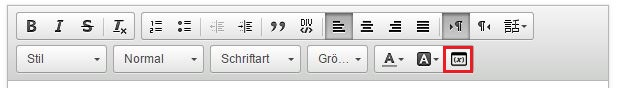
\includegraphics[scale=0.8]{ckeditor-toolbar-open-dialog}
\caption{Die \emph{CKEditor}-Funktionsleiste}
\label{fig:ckeditor-toolbar-opne-dialog}
\end{figure}
\ \newline
Die Abbildung \ref{fig:ckeditor-dialog-insert-variable} zeigt den Dialog, der vom \emph{CKEditor-Plugin} definiert und erstellt wurde. In diesem Dialog stehen alle registrierten Variablen zur Auswahl. Die Bezeichnung der Variable ist der Text in der Auswahlkomponente und die Beschreibung der ausgewählten Variable wird unterhalb der Auswahlkomponente angezeigt. Durch den Klick auf den \emph{Button OK} wird die Variable in die Vorlage eingefügt und der Dialog wird geschlossen.
\begin{figure}[h]
\centering
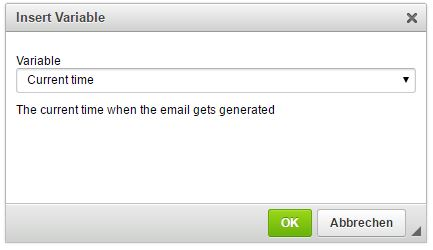
\includegraphics[scale=0.85]{ckeditor-dialog-insert-variable}
\caption{\emph{CKEditor} Dialog für die Variablenauswahl}
\label{fig:ckeditor-dialog-insert-variable}
\end{figure}
\ \newline
Die Abbildung \ref{fig:ckeditor-example-template} zeigt eine Vorlage innerhalb des \emph{CKEditors}, wobei die eingefügten Variablen besonders hervorgehoben werden. Die Bezeichnung  der Variable stellt den Namen für den \emph{HTML-Tag} bereit und die Beschreibung dessen Titel. Die eingefügten \emph{HTML-Tags} dürfen nicht verändert werden, daher ist das \emph{Drag} und \emph{Drop} und das Selektieren des eingefügten \emph{HTML-Tags} nicht erlaubt, da dadurch der eingefügte \emph{HTML-Tag} zerstört werden könnte und die Variablen nicht mehr gefunden werden können.
\begin{figure}[h]
\centering
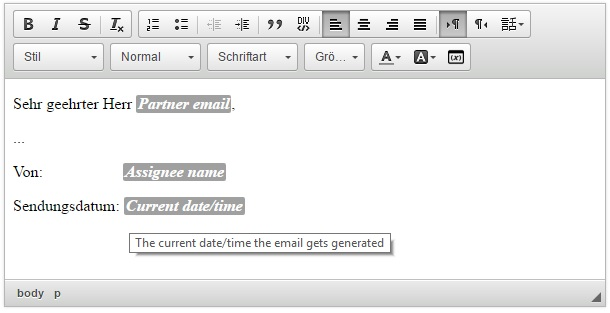
\includegraphics[scale=0.85]{ckeditor-example-template}
\caption{Beispiel einer Vorlage im \emph{CKEditor}}
\label{fig:ckeditor-example-template}
\end{figure}

\subsection{Die Implementierungen für \emph{CDI}}
\label{sec:sub-impl-integartion-cdi}
Dieser Abschnitt behandelt die Implementierungen für die Integration in eine \emph{CDI}-Umgebung, wie in Abschnitt \ref{sec:sub-template-management-cdi} beschrieben. Die Variablen werden über eine \emph{CDI}-Erweiterung gefunden und registriert und es werden die folgenden aufgelisteten Ressourcen kontextabhängig über einen implementierten \emph{CDI}-Erzeuger zur Verfügung gestellt: 
\begin{itemize}
 \item Das Objekt der Schnittstelle \emph{VariableConfiguration} 
 \newline
 ist das Objekt, dass die registrierten Variablen verwaltet.
 \item Die Objekte der Schnittstelle \emph{TemplateDataJsonBuilder}
 \newline
 sind Objekte, mit denen das \emph{JSON}-Datenobjekt für eine Vorlage und eine spezifische \emph{Template-Engine} erstellt werden kann.
 \item Die Objekte der Schnittstelle \emph{TemplateProcessor}
 \newline
 sind Objekte, mit denen Variablen in Vorlagen verwaltet werden können.
 \item Das Objekt der Klasse \emph{CdiTemplateUtil}
 \newline
 ist das Objekt mit dem die registrierten Variablen, die Objekte der Schnittstelle \emph{VariableContract} sind, in Objekte der Klasse \emph{VariableJson} konvertieren kann, wobei die Bezeichnung und die Beschreibung sprachspezifisch ermittelt werden.
\end{itemize}

\subsubsection{Die Vorlagenmanagement \emph{CDI}-Erweiterung}
Die implementierte \emph{CDI}-Erweiterung \emph{TemplateCdiExtension} findet beim Start der \emph{CDI}-Erweiterung die verfügbaren Variablen und hält die Variablen über die Lebensdauer der \emph{CDI}-Umgebung persistent. Eine \emph{CDI}-Erweiterung für eine muss folgende Voraussetzungen erfüllen, um geladen und verwendet werden zu können. 
\begin{enumerate}
	\item Sie muss die Schnittstelle \emph{javax.enterprise.inject.spi.Extension} implementieren,
	\item in einer Datei namens \emph{javax.enterprise.inject.spi.Extension}, die im Verzeichnis \emph{META-INF/services} liegen muss, mit ihren voll qualifizierten Namen registriert werden und
	\item das Artefakt, dass die \emph{CDI}-Erweiterung enthält muss eine Datei namens \emph{beans.xml} im Verzeichnis \emph{META-INF} enthalten.
\end{enumerate}
\ \newline
Die \emph{CDI}-Erweiterung wird beim Start der \emph{CDI}-Umgebung über den Mechanismus \emph{Service-Provider-Interface (SPI)} geladen und ein Objekt der Klasse der \emph{CDI}-Erweiterung erstellt. Dann kann das Objekt der \emph{CDI}-Erweiterung auf Ereignisse des Lebenszyklus der \emph{CDI}-Umgebung reagieren, in dem die \emph{CDI}-Erweiterung Beobachtermethoden für die einzelnen Ereignisse implementiert wie z.B.:
\begin{itemize}
	\item\emph{BeforeBeanDiscovery}
	\newline
	ist das Ereignis, das einmalig beim Start der \emph{CDI}-Umgebung aufgerufen wird bevor Typen, \emph{Beans} oder Injektionspunkte gesucht werden.
	\item\emph{ProcessAnnotatedType}
	\newline
	ist das Ereignis, das für jeden gefundenen injizierbaren Typ aufgerufen wird.
	\item\emph{AfterBeanDiscovery} 
	\newline
	ist das Ereignis, das einmalig Aufgerufen wird, wenn alle Typen, \emph{Beans} und Injektionspunkte gefunden und behandelt wurden.
\end{itemize}
\ \newline
Das erstellte Objekt der \emph{CDI}-Erweiterung ist an sich kein \emph{CDI-Bean}, da das Objekt der \emph{CDI}-Erweiterung bereits existiert bevor die \emph{CDI}-Umgebung vollständig gestartet wurde, ist aber trotzdem in andere \emph{CDI-Beans} injizierbar. Alle anderen \emph{CDI-Beans} können erst nachdem erfolgreichen Start der \emph{CDI}-Erweiterung injiziert werden.
\newline
\newline
Der Quelltext aus Abbildung \ref{prog:templateCdiExtension} ist ein Auszug aus der implementierten \emph{CDI}-Erweiterung \emph{TemplateCdiExtension} und zeigt die Beobachtermethoden, die auf Lebenszyklus Ereignisse der \emph{CDI}-Umgebung reagieren. Die  \emph{CDI}-Erweiterung \emph{TemplateCdiExtension} findet die Typen
\begin{itemize}
	\item alle implementierten Typen der Schnittstelle \emph{VariableContract}, die mit der Annotation \emph{CdiVariableContract} annotiert sind und
	\item alle implementierten Typen der Schnittstelle \emph{VariableResolverFactory}, die mit der Annotation \emph{CdiVariableResolverFactory} annotiert sind.
\end{itemize}
\ \newline
Die gefunden Typen werden in der \emph{CDI}-Erweiterung registriert und über die Lebensdauer der \emph{CDI}-Umgebung verwaltet. Bezüglich der Typen der Schnittstelle \emph{VariableContract} sei angemerkt, dass zur Zeit nur implementierte Typen vom Typ \emph{Enum} gefunden werden können. Alle Typen der Schnittstelle \emph{VariableContract}, die nicht vom Typ \emph{Enum} sind verursachen einen schweren Fehler und verhindern einen erfolgreichen Start der \emph{CDI}-Umgebung. Die Variablen könnten auch über implementierte Klassen der Schnittstelle \emph{VariableContract} implementiert werden und bei ihrer Verwendung dynamisch aus der \emph{CDI}-Umgebung geholt werden, was zur Zeit nicht benötigt wird.
\newline
\newline
Eine \emph{CDI}-Erweiterung ist eine injizierbare Ressource, die in jedes \emph{CDI-Bean} injiziert werden könnte, obwohl nur das Variablenmanagement sich das Objekt der \emph{CDI}-Erweiterung injizieren sollte. Es kann nicht verhindert werden, dass sich andere \emph{CDI-Beans} das Objekt der \emph{CDI}-Erweiterung injizieren lassen, da eine \emph{CDI}-Erweiterung öffentlich deklariert werden muss.

\begin{program}[h]
\caption{Auszug aus der \emph{CDI}-Erweiterung \emph{TemplateCdiExtension}}
\label{prog:templateCdiExtension}
\begin{JavaCode}
public class TemplateCdiExtension implements Extension {

    private TemplateConfiguration templateConfig;
    private Map<Class<? extends VariableContract>, 
                Class<VariableResolverFactory>>  
            variableResolverFactoryMap;

    void beforeBeanDiscovery(@Observes BeforeBeanDiscovery bbd) { ... }

    <T> void processCdiVariableContracts
             (@Observes @WithAnnotations({BaseName.class, 
                                          CdiVariableContract.class}) 
             ProcessAnnotatedType<T> pat) { ... }

    <T> void processVariableResolverFactoryFactories
        (@Observes @WithAnnotations(CdiVariableResolverFactory.class) 
        ProcessAnnotatedType<T> pat) { ... }
}
\end{JavaCode}
\end{program}
\ \newpage
\begin{itemize}
	\item\emph{beforeBeanDiscovery} 
	\newline
	ist die Beobachtermethode, die alle Objekte erstellt, die die gefundenen Typen über die Lebensdauer der \emph{CDI}-Umgebung verwalten.
	\item\emph{processCdiVariableContracts} 
	\newline
	ist die Beobachtermethode, die die gefundenen Typen der Schnittstelle \emph{VariableContract} behandelt.
	\item\emph{processVariableResolverFactoryFactories} 
	\newline
	ist die Beobachtermethode, die die gefundenen Typen der Schnittstelle \emph{VariableResolverFactory} behandelt.
\end{itemize}

\subsubsection{Der Vorlagenmanagement \emph{CDI}-Erzeuger}
Der implementierte \emph{CDI}-Erzeuger \emph{TemplateResourceProducer} produziert die kontextabhängigen Ressourcen des Vorlagenmanagements. Die Klasse \emph{TemplateResourceProducer} ist die einzige Klasse, in die das Objekt der \emph{CDI}-Erweiterung \emph{TemplateCdiExtension} injiziert wird. Im Kapitel \ref{cha:Lösungskonzept} wurde vorgegeben, dass mehrere \emph{Template-Engines} unterstützt werden müssen, daher wurde die Annotation \emph{@FreemarkerTemplate} eingeführt, die einen Injektionspunkt für die \emph{Template-Engine Freemarker} qualifiziert. In einer \emph{CDI}-Umgebung wird ein Qualifizierer benötigt, wenn für eine Schnittstelle mehrere Implementierungen zur Verfügung stehen, da ansonsten nicht entschieden werden kann welche Implementierung verwendet werden soll. Im Fall, dass es mehrere Implementierungen für eine Schnittstelle gibt, wird die Ausnahme \emph{AmbiguousResolutionException} geworfen und die \emph{CDI}-Umgebung kann nicht gestartet werden. 
\newline
\newline
Es wurden jeweils eine Erzeugermethode für den Qualifizierer \emph{@Default} und den Qualifizierer \emph{@FreemarkerTemplate} implementiert, womit nicht qualifizierte sowie qualifizierte Injektionspunkte versorgt werden können. Für die Erzeugermethode für den Qualifizierer \emph{@Default} wird die Implementierung für den Qualifizierer \emph{FreemarkerTemplate} verwendet, wodurch diese Implementierung als die Standardimplementierungen fungiert. Damit setzt man sich jedoch der Gefahr aus, dass die produzierte Standardimplementierung nicht die gewollte Implementierung ist, daher ist Vorsicht geboten, wenn diese Verhalten geändert werden sollte. 
\newline
\newline
Der Quelltext aus Abbildung \ref{prog:templateResourceProducer} ist ein Auszug aus der Klasse \emph{TemplateResourceProducer} und zeigt einige der implementierten Erzeugermethoden. 
\begin{program}[h]
\caption{Die Klasse \emph{TemplateResourceProducer}}
\label{prog:templateResourceProducer}
\begin{JavaCode}
@ApplicationScoped
public class TemplateResourceProducer implements Serializable {
    @Produces
    @ApplicationScoped
    @Default
    public VariableConfiguration produceConfiguration() {
        return extension.getVariableConfiguration();
    }
    
    @Produces
    @Dependent
    @Default
    public TemplateDataJsonBuilder produceDefaultTemplateBuilder
          (final @Default VariableResolverFactoryProvider factory) {
        return produceFreeMarkerTemplateBuilder(factory);
    }

    @Produces
    @Dependent
    @FreemarkerTemplate
    public TemplateDataJsonBuilder produceFreeMarkerTemplateBuilder
           (final @Default VariableResolverFactoryProvider factory) {
        return new FreemarkerTemplateDataJsonBuilder()
                      .withWeakMode()
                      .withVariableResolverFactoryProvider(factory);
    }
}
\end{JavaCode}
\end{program}
\ \newline
Diese beiden Methoden \emph{produceDefaultTemplateBuilder} und \emph{produceFreeMarkerTemplateBuilder} produzieren Objekte der Schnittstelle \emph{TemplateDataJsonBuilder} für den sogenannten Pseudo-\emph{Scope (@Dependent)}, wobei für jeden Injektionspunkt ein neues Objekt erstellt wird. Der Lebenszyklus von \emph{CDI-Beans} im Pseudo-\emph{Scope} wird nicht von der \emph{CDI}-Umgebung verwaltet und die Lebensdauer eines \emph{CDI-Bean} im Pseudo-\emph{Scope} ist gebunden and das \emph{CDI-Bean}, das sich das Pseudo-\emph{Scoped} \emph{CDI-Bean} injiziert hat. Die Erzeugermethoden \emph{produceDefaultTemplateBuilder} und \emph{produceFreeMarkerTemplateBuilder} lassen sich als Argument ein Objekt der Schnittstelle \emph{VariableResolverFactoryProvider} injizieren, dessen Geltungsbereich für diese Methoden nicht bekannt ist.
\newline
\newline
Die Methode \emph{produceConfiguration} produziert ein Objekt der Schnittstelle  \emph{VariableConfiguration}, das die registrierten Variablen enthält und von der \emph{CDI}-Erweiterung bereitgestellt wird. Nachdem die Schnittstelle  \emph{VariableConfiguration} nur lesenden Zugriff erlaubt, wird dieses Objekt für den Gültigkeitsbereich der Anwendung produziert, also einmalig für die gesamte Lebensdauer der \emph{CDI}-Umgebung.
\newline
\newline
Alle injizierbaren Objekte werden erst beim ersten Zugriff auf eine ihrer öffentlichen Methoden erzeugt und im korrespondierenden Geltungsbereich registriert. Sollte ein injizierbares Objekt niemals verwendet werden, so wird es auch niemals erzeugt. Dieses Verhalten ist möglich, da alle Injektionspunkte von \emph{Proxies} verwaltet werden, die beim Starten der \emph{CDI}-Umgebung in die Injektionspunkte injiziert werden und ein abgeleiteter Typ des injizierten Typs sind. Bei einem Zugriff auf eine öffentliche Methode des injizierten Objekts, wird das korrespondierende Objekt aus den aktuellen Geltungsbereich geholt und der Aufruf an dieses Objekt weiter delegiert.  

\subsubsection{Die Vorlagenmanagement \emph{CDI}-Hilfsklasse}
Die Klasse \emph{CdiTemplateUtil} aus dem Quelltext aus Abbildung \ref{prog:cdiTemplateUtil} wurde implementiert, um ein injizierbares \emph{CDI-Bean} zur Verfügung zu stellen, das Hilfsmethoden für die Konvertierung der Variablen von Objekten der Schnittstelle \emph{VariableContract} in Objekte der Klasse \emph{VariableJson} und visa versa zur Verfügung stellt. Diese Implementierung hält keinen Status, daher kann dieses \emph{CDI-Bean} in den Geltungsbereich der Anwendung registriert werden. Die Verwendung des Objekts der Klasse \emph{CdiTemplateUtil} ist \emph{Thread-Safe}
\begin{itemize}
	\item da kein Status in diesem Objekt gehalten wird und
	\item das verwendete Objekt der Klasse \emph{TemplateConfiguration} nur lesenden Zugriff erlaubt.
\end{itemize}
\ \newline
Die Annotation \emph{@Typed(CdiTemplateUtil.class)} bewirkt dass dieses \emph{CDI-Bean} nur über den Typ \emph{CdiTemplateUtil} injizierbar ist. Mit der Annotation \emph{@Typed} kann man einschränken, über welche Typen ein \emph{CDI-Bean} injizierbar ist, was hilfreich ist, wenn die Klasse eines \emph{CDI-Beans} mehrere Schnittstellen implementiert.

\begin{program}[h]
\caption{Die Klasse \emph{CdiTemplateUtil}}
\label{prog:cdiTemplateUtil}
\begin{JavaCode}
@ApplicationScoped
@Typed(CdiTemplateUtil.class)
public class CdiTemplateUtil implements Serializable {

    @Inject
    private VariableConfiguration config;

    public List<VariableJson> convertContractToJsonModel
    						  (final Locale locale) { }

    public List<VariableJson> convertContractToJsonModel
    		(final Collection<VariableContract> contracts,
             final Locale locale) { }

    public VariableJson convertContractToJsonModel
           (final VariableContract contract,
            final Locale locale) { }
	
    public List<VariableContract> convertJsonModelToContract
    							 (final Collection<VariableJson> jsonModels) { }

    public VariableContract convertJsonModelToContract
                            (final VariableJson jsonModel) { }
}
\end{JavaCode}
\end{program}

\subsection{Die Implementierungen für \emph{JSF}}
\label{sec:sub-impl-integartion-jsf}
Dieser Abschnitt behandelt die Implementierung des Variablenmanagements für die \emph{View}-Technologie \emph{JSF}. In diesem Abschnitt wird sich nur dem implementierten \emph{FacesConverter} und der \emph{CKEditor}-Integration, bereitgestellt von \emph{primefaces-extensions}, beschäftigen.

\subsubsection{Der Vorlagen \emph{FacesConverter}}
Es wurde der Konverter \emph{AbstractTemplateConverter} als abstrakte Klasse implementiert, die die Schnittstelle \emph{javax.faces.Converter} implementiert. Diese abstrakte Klasse wurde implementiert, da die Logik für die Konvertierung0 über alle \emph{Template-Engines} dieselbe ist und sich lediglich die Implementierung der Schnittstelle \emph{TemplateProcessor} unterschiedet. Das Objekt der Schnittstelle \emph{TemplateProcessor} und das Objekt der Klasse \emph{CdiTemplateUtil} werden manuell von der \emph{CDI}-Umgebung geholt, da keine Injektion innerhalb von \emph{JSF}-Artfakten in \emph{JSF 2.2} möglich ist. Die Injektion in \emph{JSF}-Artefakte wird erst ab \emph{JSF 2.3} unterstützt werden. Die Objekte werden über die Klasse \emph{BeanProvider} der Bibliothek \emph{Deltaspike} geholt, die Hilfsmethoden zur Verfügung stellt, mit denen man zur Laufzeit manuell mit der \emph{CDI}-Umgebung interagieren kann. \emph{Deltaspike} ist eine Bibliothek, die eine portable \emph{CDI}-Erweiterung darstellt. 
\newline
\newline
Die konkrete Implementierung \emph{FreemarkerTemplateConverter} für die \emph{Template-Engine Freemarker}, die von der abstrakten Klasse \emph{AbstractTemplateConverter} ableitet, setzt über einen Konstruktor in der Basisklasse den korrespondierenden Qualifizierer für die verwendete \emph{Template-Engine} und das zu verwendende Objekt der Klasse \emph{java.util.Locale}. Mit diesem Qualifizierer wird die korrekte Implementierung der Schnittstelle \emph{TemplateProcessor} aus dem \emph{CDI-Container} geholt. Da der Konverter eine Abhängigkeit auf ein \emph{Locale} Objekt besitzt, muss ein Objekt des Konverters im \emph{Quelltext} erzeugt und über Parameterbindung an eine \emph{JSF}-Komponente gebunden werden. Das Binden des Konverters an eine \emph{JSF}-Komponente über dessen Namen definierbar über die Annotation \emph{@FacesConverter("converterName")} ist nicht möglich. 

\begin{program}[h]
\caption{Die Klasse \emph{FreemarkerTemplateConverter}}
\label{prog:freemarkerTemplateConverter}
\begin{JavaCode}
public class FreemarkerTemplateConverter 
                          extends AbstractTemplateConverter {

    public FreemarkerTemplateConverter(final Locale locale) {
        super(new FreemarkerTemplateLiteral(), locale);
    }
}
\end{JavaCode}
\end{program}
\ \newline
Die abstrakte Klasse \emph{AbstractTemplateConverter} definiert reguläre Ausdrücke, um die Variablen einer Vorlage in Form von \emph{HTML-Tags} zu finden und zu konvertieren.
\begin{JavaCode}[numbers=none]
String tagRegex = "(<span[^,>]*class=\"variable\"[^,>]*>[^,<]*</span>)";
String idRegex  = "data-variable-id=\"(\\S+)\"";
\end{JavaCode}
\ \begin{itemize}
	\item\emph{tagRegex} ist der reguläre Ausdruck, um die Variablen in ihrer \emph{HTML}-Repräsentation in einer Vorlage zu finden.
	\item\emph{idRegex} ist der reguläre Ausdruck, um die \emph{Id} einer Variable, aus deren \emph{HTML}-Repräsentation zu bekommen und wird auf den gefundenen \emph{HTML-Tag} einer Variable angewendet, die mit dem regulären Ausdruck \emph{tagRegex} gefunden wurde.
\end{itemize}
\ \newline
Die abstrakte Klasse \emph{AbstractTemplateConverter} definiert auch eine Vorlage in Form einer Zeichenkette, mit der die Variablen in ihre \emph{HTML-Tag}-Repräsentation konvertiert werden können, wobei diese Vorlage unabhängig von der verwendeten \emph{Template-Engine} ist und auf alle Variablen gleich angewendet werden kann.
\begin{JavaCode}
String template = "<span class=\"variable\" contentEditable=\"false\" "
                + "data-variable-id=\"{0}\" title=\"{1}\">{2}</span>";
\end{JavaCode}
Die Vorlage \emph{template} wird mit \emph{java.text.MessageFormat(String, Object...)} verarbeitet, wobei der Formalparameter \emph{Object...}, der eine variable Argumentliste repräsentiert, über den die dynamischen Werte für die Vorlage bereitgestellt werden können. 

\subsubsection{Die \emph{Primefaces-Extension} für den \emph{CKEditor}}
Der \emph{Rich-Editor CKEditor} ist eine \emph{Javascript} basierte Anwendung, die nur am \emph{Browser} der BenutzerInnen läuft. Es wird aber eine \emph{JSF}-Integration benötigt, damit man
\begin{itemize}
	\item auf \emph{AJAX-Events} reagieren kann,
	\item\emph{FacesConverter} verwenden kann und
	\item Parameterbindungen definieren kann.
\end{itemize}
\ \newline
Da es nicht trivial ist eine vollwertige \emph{JSF}-Komponente zu implementieren und das Implementieren einer solchen Komponente auch viel Zeit in Anspruch nimmt, wurde auf die Implementierung von \emph{Primefaces-Extensions} zurückgegriffen, die bereits eine vollwertige \emph{JSF}-Integration für den \emph{CKEditor} bereitstellt. \emph{Primefaces-Extensions} ist eine quelloffene Bibliothek, die die quelloffene Bibliothek \emph{Primefaces} erweitert. \emph{Primefaces} ist zurzeit eine der bekanntesten \emph{JSF}-Komponenten Bibliothek im \emph{Java}-Umfeld.
\newline
\newline
Die Ressourcen für den \emph{CKEDitor} bewegen sich in der Größenordnung von 1,5 Megabyte, daher werden die Ressourcen in einem separaten Artefakt zur Verfügung gestellt. Man kann auch eine eigene Implementierung zur Verfügung stellen, sofern diese Implementierung in derselben  Version vorhanden ist, wie von \emph{Primefaces-Extensions} unterstützt wird. Der \emph{CKEditor} ist ein sehr umfangreicher \emph{Editor}, den man sich auch seinen Wünschen entsprechend selbst zusammenstellen kann. Eine solche benutzerdefinierte Zusammenstellung des \emph{CKEditors} kann man heranziehen, um die Standardimplementierung zu ersetzen.
\newline
\newline
Der Quelltest aus Abbildung \ref{prog:example-ckeditor-xhtml} illustriert die Verwendung des \emph{CKEditors} in Form der zur Verfügung gestellten \emph{JSF}-Komponente.
\begin{program}[h]
\caption{\emph{XHTML-Markup} für \emph{CKEditor}}
\label{prog:example-ckeditor-xhtml}
\begin{HtmlCode}
<pe:ckEditor id="template_content_editor"
             wdgetVar="pfEditor"
             value="#{templateEditModel.content}"
             converter="#{ckeditorBean.converter}" 
             contentsCss="resources/css/myStyle.css"
             customConfig="./ckeditor-config.js">
</pe:ckEditor>
\end{HtmlCode}
\end{program}
\ \begin{itemize}
	\item\emph{id} ist das Attribute, um die eindeutige \emph{Id} innerhalb des Namensraums der Komponente zu definieren.
	\item\emph{widgetVar} ist das Attribut, um einen eindeutigen Name des \emph{Javascript}-Objekts, das den Zugriff auf den \emph{CKEditor} in \emph{Javascript} erlaubt, zu definieren.
	\item\emph{value} ist das Attribut, um die Parameterbindung der Vorlage zu einem \emph{Java}-Objekt zu definieren.
	\item\emph{converter} ist das Attribut, um den verwendeten Konverter, der die Vorlagen konvertiert, über Parameterbindung zu setzen.
	\item\emph{contentCss} ist das Attribut, um eine eigene \emph{CSS}-Datei für den Inhalt der Vorlage zu definieren. Die Vorlage wird innerhalb des \emph{Editors} als eigenständige \emph{HMTL}-Datei behandelt, das in einer \emph{Iframe}-Komponente gehalten wird.
	\item\emph{customConfig} ist das Attribut, um die eigene Konfiguration des \emph{Editors} in Form von einer eigenen \emph{Javascript}-Datei zu definieren. 
\end{itemize}

\section{Die Vorlagenmanagement Beispielanwendung}
Der folgende Abschnitt beschäftigt sich mit der implementierten Beispielanwendung, für das Vorlagenmanagement, die die Verwendung des Vorlagenmanagement im Bezug auf 
\begin{itemize}
	\item die Verwendung in der Geschäftslogik,
	\item die Verwendung über eine Webseite und
	\item die Verwendung zum Erstellen einer \emph{E-Mail}  
\end{itemize}
aufzeigen soll. Dazu wurde eine Demowebanwendung implementiert, die die Web seitige  Verwaltung der Vorlagen implementiert. Es wurde auch eine Klasse implementiert, die aufzeigen soll, wie eine \emph{E-Mail} basierend auf einer Vorlage, aus einer Geschäftslogik heraus erstellt werden kann. 

\subsection{Die Verwendung in einem \emph{Business}-Service}
Der folgende Quelltext aus Abbildung \ref{prog:emailServiceCdiEventImpl} zeigt wie eine \emph{E-Mail} über die die implementierte Klasse \emph{EmailServiceImpl} der Schnittstelle \emph{EmailService} erstellt werden kann. Das Objekt der Schnittstelle \emph{EmailService} wird über die \emph{CDI}-Umgebung zur Verfügung gestellt und mittels Injektion in die Geschäftslogik injiziert. Die Schnittstelle \emph{EmailService} und dessen Implementierung \emph{EmailServiceCdiEventImpl} befinden sich im Artefakt \emph{mailing-template-integration-clevercure-web}. Dieses Artefakt stellt die Integration in die Anwendung \emph{CleverWeb}  dar. Die \emph{E-Mails} werden in der Implementierung \emph{EmailServiceCdiEventImpl} über \emph{CDI-Events} erstellt, damit ist die Logik für das Erstellen der \emph{E-Mail} vollständig entkoppelt von dieser Implementierung. Im folgenden sind die zur Verfügung gestellten Methoden der Schnittstelle \emph{EmailService} angeführt, die der Geschäftslogik zur Verfügung stehen.
\begin{itemize}
	\item\emph{public void create(EmailDTO dto)}
	\newline
	ist die Methode, mit der eine \emph{E-Mail} sofort erstellt werden können.
	\item\emph{public void create(List<EmailDTO> dtos)}
	\newline
	ist die Methode, mit der mehrere \emph{E-Mails} sofort erstellt werden können.
	\item\emph{public void createAfterSuccess(EmailDTO dto)}
	\newline
	ist die Methode, mit der eine \emph{E-Mail} nach dem erfolgreichem Beenden einer Transaktion erstellt werden kann.
	\item\emph{public void createAfterSuccess(List<EmailDTO> dto)}
	\newline
	ist die Methode, mit der mehrere \emph{E-Mails} nach dem erfolgreichem Beenden einer Transaktion erstellt.
 werden kann.    
\end{itemize} 
\begin{program}[h]
\caption{EmailServiceCdiEventImpl.java}
\label{prog:emailServiceCdiEventImpl}
\begin{JavaCode}
@RequestScoped
@Transactional(Transactional.TxType.SUPPORTS)
public class EmailServiceCdiEventImpl implements EmailService {
    @Inject
    private Event<CreateEmailsEvent<CreateEmailsEvent.CreateImmediate>> createImmediateEvent;
    @Inject
    private Event<CreateEmailsEvent<CreateEmailsEvent.CreateAfterSuccess>> createAfterSuccessEvent;
    @Inject
    private Event<CreateEmailsEvent<CreateEmailsEvent.CreateAfter>> createAfterEvent;

    @Override
    @Transactional(Transactional.TxType.REQUIRED)
    public void create(EmailDTO dto) {
        createImmediateEvent.fire(new CreateEmailsEvent<>(dto));
    }

    @Override
    @Transactional(Transactional.TxType.REQUIRED)
    public void create(List<EmailDTO> dtos) {
        createImmediateEvent.fire(new CreateEmailsEvent<>(dtos));
    }

    @Override
    public void createAfterSuccess(EmailDTO dto) {
        createAfterSuccessEvent.fire(new CreateEmailsEvent<>(dto));
    }

    @Override
    public void createAfterSuccess(List<EmailDTO> dtos) {
        createAfterSuccessEvent.fire(new CreateEmailsEvent<>(dtos));
    }
}
\end{JavaCode}
\end{program}
\ \newline
Der Quelltext aus Abbildung \ref{prog:businessServiceImpl} zeigt das Beispiel der Geschäftslogik, die über die Schnittstelle \emph{EmailService} \emph{E-Mails} erstellt. Die zu erstellende \emph{E-Mail} wird durch ein Objekt der Klasse \emph{EmailDTO} repräsentiert, das alle benötigten Informationen für das Erstellen einer \emph{E-Mail} enthält.
\newpage
\begin{program}[h]
\caption{BusinessServiceImpl.java}
\label{prog:businessServiceImpl}
\begin{JavaCode}
@RequestScoped
@Transactional(Transactional.TxType.REQUIRED)
public class BusinessServiceImpl implements BusinesService {

    @Inject
    private EmailService emailService;

    @Override
    public void doBusinessEmailImmediate() {
        emailService.create(createEmailDto());
    }

    @Override
    public void doBusinessEmailAfterSuccess() {
        emailService.createAfterSuccess(createEmailDto());
    }

    private EmailDTO createEmailDto() {
        final String email = "herzog.thomas8@gmail.com";
        final Long mailUserId = 1L;
        final List<Long> mailTypeIds = Collections.singletonList(1L);
        final Locale locale = Locale.US;
        final ZoneId zone = ZoneId.systemDefault();
        final Map<Object, Object> userData = 
        	new HashMap<Object, Object>() {{
                put(TemplateVariable.SENDER_USER, "Thomas Herzog");
                put(TemplateVariable.RECIPIENT_USER, "Hugo Maier");
                put(TemplateVariable.TOPIC, "User status changed");
                put(TemplateVariable.STATUS, "Inactive");
            }};
        return new EmailDTO(email, 
        					locale, 
        					zone, 
        					mailUserId, 
        					userData, 
        					mailTypeIds);
    }
}
\end{JavaCode}
\end{program}
\ \newline
Folgende Auflistung erklärt die Attribute, die beim Erstellen eine Objekts der Klasse \emph{EmailDto} angegeben werden müssen.
\begin{itemize}
	\item\emph{email} ist die Zeichenkette, die die \emph{E-Mail}-Adresse definiert.
	\item\emph{mailUserId} ist die \emph{Id} des virtuellen Benutzers, der die \emph{E-Mail} auf der Datenbank erstellt.
	\item\emph{mailTypeIds} ist die Menge von \emph{Ids}, die die \emph{Mail}-Typen repräsentieren. Jedem \emph{Mail}-Typ ist eine Voralge zugeordnet.
	\item\emph{locale} ist das Objekt der Klasse \emph{java.util.Locale} , das die Sprache definiert.
	\item\emph{zone} ist das Objekt der Klasse \emph{java.time.ZoneId}, das die Zone für die Datumsformatierung definiert.
	\item\emph{userData} ist der assoziative Behälter, der die Benutzerdaten enthält, die bei der Evaluierung verwendet werden.
\end{itemize}

\subsection{Die Verwendung über eine \emph{Web}-Oberfläche}
Die Abbildung \ref{fig:demo_web_app_empty_view_part_1} zeigt die Weboberfläche, die für die Beispielanwendung implementiert wurde. Über dieses Formular können die Voralgen sprachspezifisch verwaltet werden.
\ \begin{figure}[h]
\centering
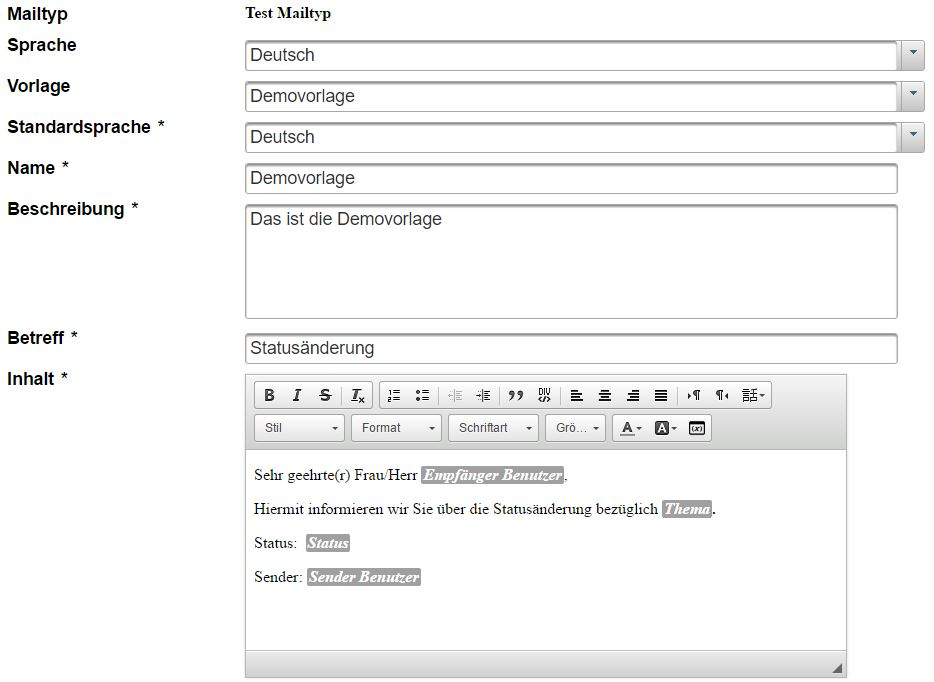
\includegraphics[scale=0.5]{demo_web_app_empty_view_part_1}
\caption{Formular für die Verwaltung der Vorlagen}
\label{fig:demo_web_app_empty_view_part_1}
\end{figure}
\ \newline
Die Abbildung \ref{fig:demo_web_app_empty_view_part_2} zeigt, den Teil der Webseite, der die relevanten Daten einer Vorlage anzeigt.
\begin{itemize}
	\item\emph{Decorator Template} ist die \emph{Freemarker}-Voralge, die von jeder Vorlage dekoriert wird.
	\item\emph{User Template} ist die Vorlage, die von einem BenutzerIn erstellt wurde.
	\item\emph{Template JSON Data} ist die \emph{JSON}-Zeichenkette, die erstellt wird, wenn die Daten für eine Vorlage serialisiert werden.
	\item\emph{Parsed Template} ist die Vorlage, in der die Variablen durch die serialisierten Werte ersetzt wurden.
	\item\emph{Template Metadata} sind die Metadaten der Vorlage, wie z.B. die Anzahl der enthalten Variablen.
\end{itemize}
\begin{figure}[h]
\centering
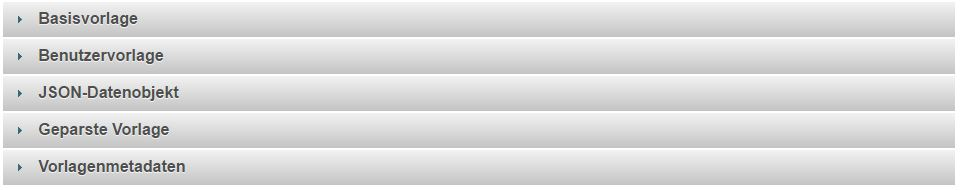
\includegraphics[scale=0.5]{demo_web_app_empty_view_part_2}
\caption{Anzeige der aller relevanten Daten einer Vorlage}
\label{fig:demo_web_app_empty_view_part_2}
\end{figure}

\subsubsection{Die dekorierbare Vorlage}
Die Abbildung \ref{fig:demo_web_app_data_decorator} zeigt die dekorierbare \emph{Freemarker}-Vorlage, die alle Vorlagen dekorieren. Sie stellt den \emph{HTML-Body} zur Verfügung, da die Benutzervoralgen nur den Inhalt innerhalb des \emph{HTML-Tags body} bereitstellen.
\begin{figure}[h]
\centering
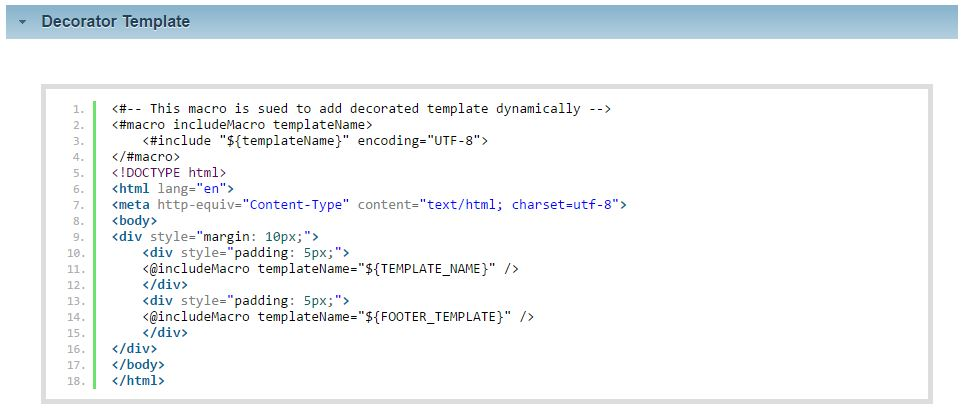
\includegraphics[scale=0.5]{demo_web_app_data_decorator}
\caption{Das \emph{Decorator Template}}
\label{fig:demo_web_app_data_decorator}
\end{figure}
\ \newpage

\subsubsection{Die Benutzervorlage}
Die Abbildung \ref{fig:demo_web_app_data_template} zeigt die \emph{Freemarker}-Vorlage, die von der BenutzerInnen erstellt wird. Die Vorlage enthält zwar \emph{HTML-Markup}, aber nur den Inhalt unterhalb des \emph{HTML-Tags body}. Sie stellt aber kein vollständiges \emph{HTML}-Dokument zur Verfügung.
\begin{figure}[h]
\centering
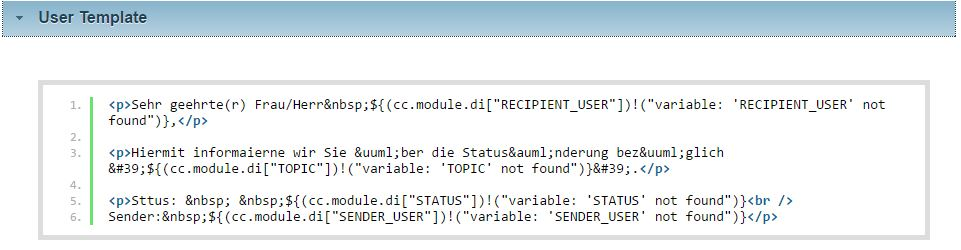
\includegraphics[scale=0.5]{demo_web_app_data_template}
\caption{Die \emph{Benutzervorlage} als \emph{Freemarker Template}}
\label{fig:demo_web_app_data_template}
\end{figure}

\subsubsection{Die serialisierte \emph{JSON}-Zeichenkette}
Die Abbildung \ref{fig:demo_web_app_data_json} zeigt die serialisierte \emph{JSON}-Zeichenkette, die beim Erstellen einer \emph{E-Mail} erstellt wird und in der Datenbank persistent gehalten wird. Mit diesen Daten kann eine \emph{E-Mail} auf Basis dieser Vorlage jederzeit wiederhergestellt werden.
\begin{figure}[h]
\centering
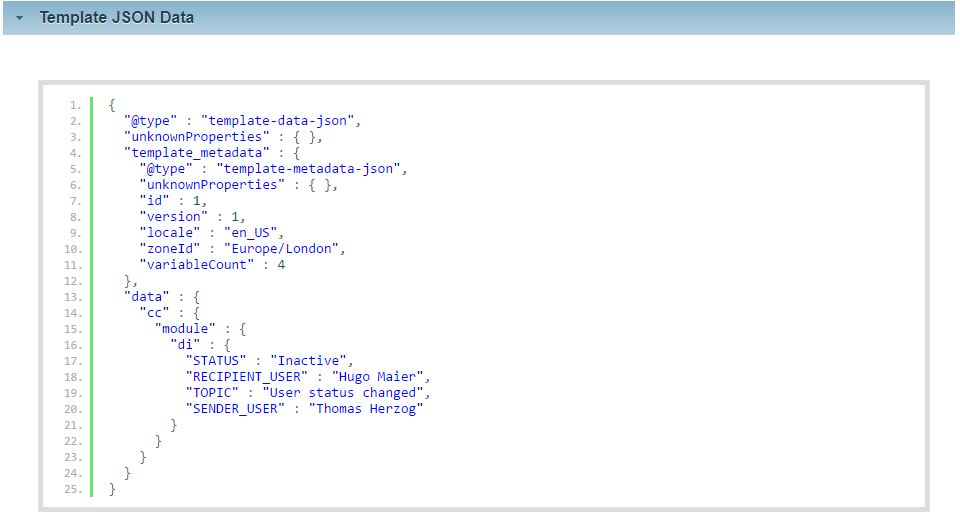
\includegraphics[scale=0.5]{demo_web_app_data_json}
\caption{Der serialisierte \emph{JSON}-String}
\label{fig:demo_web_app_data_json}
\end{figure}
\ \newpage

\subsubsection{Die Vorlagenmetadaten}
Die Abbildung \ref{fig:demo_web_app_data_metadata} zeigt die Metadaten der Benutzervorlage. Die Metadaten sind nur für die Entwicklung relevant.
\begin{figure}[h]
\centering
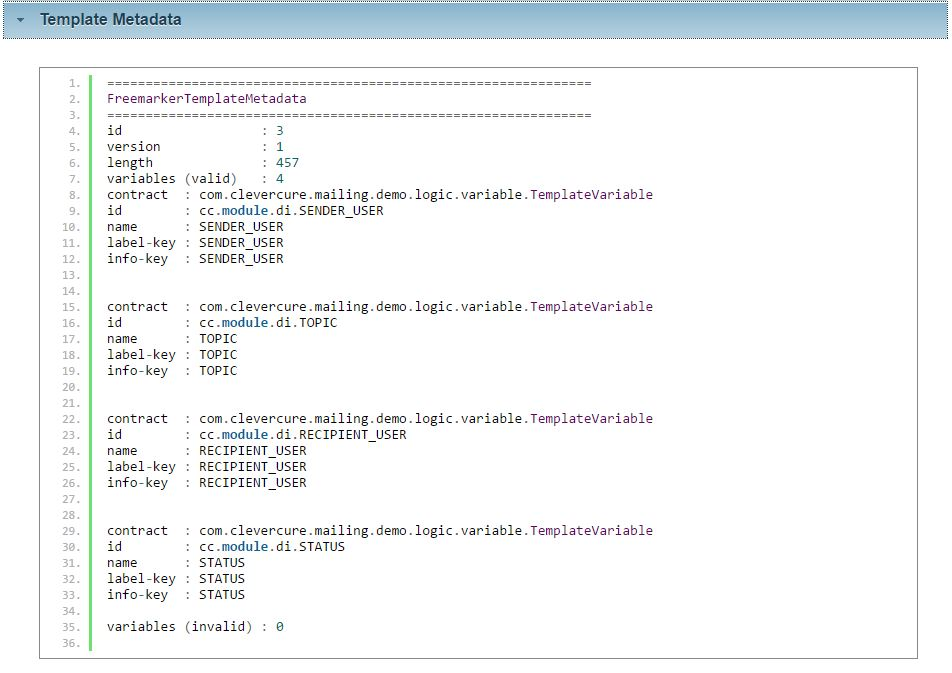
\includegraphics[scale=0.5]{demo_web_app_data_metadata}
\caption{Die Metadaten der Vorlage}
\label{fig:demo_web_app_data_metadata}
\end{figure}

\subsubsection{Der erstellte \emph{E-Mail}-Inhalt}
Die Vorlage mit den aufgelösten Variablen aus Abbildung \ref{fig:demo_web_app_data_parsed} zeigt die Metadaten der Benutzervorlage. 
\begin{figure}[h]
\centering
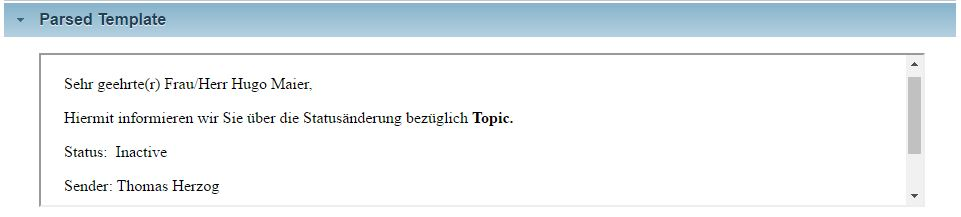
\includegraphics[scale=0.5]{demo_web_app_data_parsed}
\caption{Die Metadaten der Vorlage}
\label{fig:demo_web_app_data_parsed}
\end{figure}
\chapter{Die Analyse und Tests}
\label{cha:Analyse}
Dieses Kapitel beschäftigt sich mit der Analyse der Implementierung und dessen Tests. Es gibt zwei Arten von Tests die implementiert wurden
\begin{itemize}
	\item die \emph{JUnit}-Tests sind die Tests, die nicht auf eine \emph{CDI}-Umgebung angewiesen sind und 
	\item die \emph{CDI-JUnit}-Tests sind die Tests, die auf eine \emph{CDI}-Umgebung angewiesen sind.
\end{itemize}

\section{Die Tests}
Dieser Abschnitt beschäftigt sich mit den Implementieren Tests des Vorlagenmanagements und der Implementierten Konfiguration für die Tests. Für die Tests wurden folgende Bibliotheken verwendet.
\begin{itemize}
	\item\emph{JUnit4} ist ein \emph{Framework}, mit dem wiederholbare Tests implementiert werden können und ist als Standard für Tests in \emph{Java} anzusehen.
	\item\emph{Deltaspike} ist ein \emph{Open-Source}-Projekt der \emph{Apache Software Foundation (ASF)}, die portable \emph{CDI}-Erweiterungen in Form von Modulen bereitstellt und auch eine Erweiterung für \emph{JUnit}-Tests bereitstellt, mit denen Tests in einer \emph{CDI}-Umgebung lauffähig sind.
\end{itemize}
\ \newline
Alle implementierten Tests sind nicht auf einen Anwendungsserver angewiesen und sind innerhalb des lokalen Klassenpfades lauffähig und können daher in jeder Entwicklungsumgebung und bei einem Kompilieren über das \emph{Buildtool Maven} ausführbar.
\newline
\newline
Die Tests wurden wie folgt organisiert.
\begin{itemize}
	\item\emph{com.clevercure.mailing.test.*} 
	\newline
	ist das \emph{Java}-Paket in dem alle implementierten Tests liegen. 
	\item\emph{*.[toTestClass]Tests}
	\newline
	ist das \emph{Java}-Paket, für eine zu testende Klasse, wobei der Paketname den Namen der zu testenden Klasse mit dem Suffix Tests enthält.
	\item\emph{[toTestMethod]Test.java}
	\newline
	ist die implementierte Testklasse für die Tests einer Methode der zu testenden Klasse.
	\item\emph{test\_case}
	\newline
	ist der Name der einzelnen Testmethoden, der wiedergibt was an einer Methode getestet wird. 
\end{itemize}
\ \newline
Die vorgestellte Konvention der Tests wurde so umgesetzt sofern es möglich war. 

\subsection{Die Tests der \emph{CDI}-Erweiterung}
Die Tests aus Abbildung \ref{fig:tests-template-cdi} testen die Implementierungen des Artefakts \emph{mailing-moule-template-cdi} wie
\begin{itemize}
	\item den Klasse \emph{TemplateCdiExtension},
	\item die Klasse \emph{CdiTemplateUtils} und
	\item die Klasse \emph{TemplateResourceProducer}.
\end{itemize}
\begin{figure}[h]
\centering
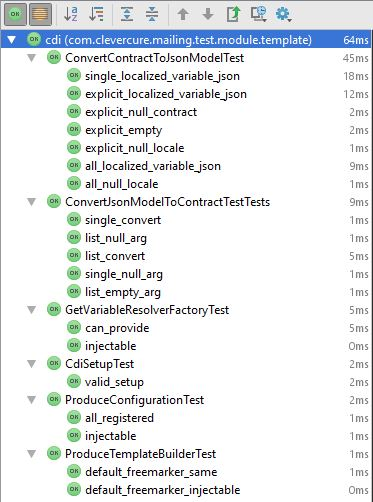
\includegraphics[scale=0.8]{tests-template-cdi}
\caption{Testdurchlauf der Tests der \emph{CDI}-Erweiterung}
\label{fig:tests-template-cdi}
\end{figure}
\ \newpage

\subsection{Die Tests der \emph{Web}-Oberfläche}


\section{Die erreichten Ziele}

\subsection{Das Vorlagen-\emph{Management über \emph{CKEditor}}}

\subsection{Das Vorlagen-\emph{Management} in einer \emph{CDI}-Umgebung}

\subsection{Das Vorlagen-\emph{Management} in JSF}
\subsection{Das Vorlagen-\emph{Management} in \emph{Mail}-DB-Schema}



%%%----------------------------------------------------------
%%%Anhang
\appendix
\chapter{Technische Informationen}
\label{ch:TechnischeInfos}

\newcommand*{\checkbox}{{\fboxsep 1pt%
\framebox[1.30\height]{\vphantom{M}\checkmark}}}

\section{Aktuelle Dateiversionen}

\begin{center}
\begin{tabular}{|l|l|}
\hline
Datum & Datei \\
\hline\hline
\hgbthesisDate & \texttt{hgbthesis.cls} \\
\hline
\hgbDate       & \texttt{hgb.sty} \\
\hline
\end{tabular}
\end{center}




\section{Details zur aktuellen Version}


Das ist eine völlig überarbeitete Version der DA/BA-Vorlage, die
\mbox{UTF-8} kodierten Dateien vorsieht und ausschließlich im PDF-Modus arbeitet.
Der "`klassische"' DVI-PS-PDF-Modus wird somit nicht mehr unterstützt! 

\subsection{Allgemeine technische Voraussetzungen}

Eine aktuelle \latex-Installation mit
\begin{itemize}
	
		\item Texteditor für \mbox{UTF-8} kodierte (Unicode) Dateien,
		\item \texttt{biber}-Programm (BibTeX-Ersatz, Version $\geq 1.5$),
		\item \texttt{biblatex}-Paket (Version $\geq 2.5$, 2013/01/10),
		\item Latin Modern Schriften (Paket \texttt{lmodern}).%
			\footnote{\url{http://www.ctan.org/pkg/lm}, \url{http://www.tug.dk/FontCatalogue/lmodern}}
\end{itemize}


\subsection{Verwendung unter Windows}

Eine typische Installation unter Windows sieht folgendermaßen aus
(s.\ auch Abschnitt \ref{sec:Windows}):
%
\begin{enumerate}
\item \textbf{MikTeX 2.9}%
	\footnote{\url{www.miktex.org} -- \textbf{Achtung:} 
	Generell wird die \textbf{Komplett\-installation} von MikTeX ("`Complete MiKTeX"') empfohlen, 
	da diese bereits alle notwendigen Zusatzpakete und Schriftdateien enthält! 
	Bei der Installation ist darauf zu achten, 
	dass die automatische Installation erforderlicher Packages 
	durch "`\emph{Install missing packages on-the-fly: = Yes}"' ermöglicht wird (NICHT "`\emph{Ask me first}"')!
	Außerdem ist zu empfehlen, unmittelbar nach der Installation von MikTeX mit dem Programm
	\texttt{MikTeX} $\to$ \texttt{Maintenance} $\to$ \texttt{Update} und \texttt{Package Manager} 
	ein Update der installierten Pakete durchzuführen.}
	(zurzeit am einfachsten die 32-Bit Version, da nur diese das Programm \texttt{biber.exe} 
	bereits enthält),
\item \textbf{TeXnicCenter 2.0}%
	\footnote{\url{http://www.texniccenter.org/}}
	(Editor-Umgebung, unterstützt UTF-8),
\item \textbf{SumatraPDF}%
	\footnote{\url{http://blog.kowalczyk.info/software/sumatrapdf/}} 
	(PDF-Viewer),
\end{enumerate}
%
Ein passendes TeXnicCenter-Profil für MikTeX, Biber und Sumatra ist in diesem Paket enhalten
(Datei \verb!_tc_output_profile_sumatra_utf8.tco!). Dieses sollte man zuerst
über \texttt{Build} $\to$ \texttt{Define Output Profiles} in TeXnicCenter importieren.
\textbf{Achtung}: Alle neu angelegten \texttt{.tex}-Dateien sollten in UTF-8 Kodierung gespeichert werden!




\subsection{Verwendung unter Mac~OS}


Diese Version sollte insbesondere mit \emph{MacTeX} problemlos laufen (s.\ auch Abschnitt \ref{sec:MacOs}):
\begin{enumerate}
\item 
	\emph{MacTex} (2012 oder höher).
\item 
	Die Zeichenkodierung des Editors sollte auf UTF-8 eingestellt sein.
\item 
	Als Engine (vergleichbar mit den Ausgabeprofilen in TeXnicCenter) sollte \emph{LaTeXMk} verwendet werden. 
	Dieses Perl-Skript erkennt automatisch, wie viele Aufrufe von \emph{pdfLaTeX} und \emph{Biber} nötig sind. 
	Die Ausgabeprofile \emph{LaTeX} oder \emph{pdfLaTeX} hingegen müssen mehrmals aufgerufen werden, 
	zudem werden hierbei auch die Literaturdaten nicht verarbeitet. Dazu müsste extra die \emph{Biber}-Engine 
	aufgerufen werden, 	die jedoch noch nicht in allen Editoren vorhanden ist.
\end{enumerate}


\begin{comment}
\subsection{Vorteile}
\begin{itemize}
\item PDF wird direkt erzeugt ohne DVI und PS; damit ist angeblich auch die "`Feintypographie"' besser.
\item Die Verwendung von \texttt{SumatraPDF} erlaubt funktionierende Forward- und Inverse-Suche, womit erstmals ein effektiver PDF-Workflow möglich ist.
\item Preview der vollständigen Manuskripts (inklusive Grafiken) ist in PDF viel schneller
als in DVI (mit YAP und Ghostscript für die Grafiken).
\item Grafiken können auch als PDF, PNG oder JPEG direkt eingebunden werden. Bestehende EPS-Grafiken werden automatisch in PDF konvertiert. 
\item Bei eingebundenen Rasterbildern werden (im Unterschied zu \texttt{ps2pdf} in der Default-Einstellung) keine zusätzlichen JPEG-Artefakte erzeugt. 
(Anmerkung: im TC-Ausgabeprofil für \texttt{ps2pdf} ist dafür jetzt die
Option \verb!-dPDFSETTINGS=/prepress! eingestellt -- \verb!=/printer! ist nicht ausreichend!)
\item Die Erzeugung von aktiven Verweisen mit \texttt{hyperref} funktioniert problemlos, mit allen Vorteilen (einschließlich der Zeilenumbrüche in URLs).
\item PDF-Metadaten (zur verbesserten Suche) werden direkt aus den Dokumentendaten durch LaTeX generiert.
\end{itemize}

\subsection{Weitere Neuerungen}
%
\begin{sloppypar}
\begin{itemize}
\item Verwendung des \texttt{epstopdf}-Pakets, wodurch vorhandene EPS-Grafiken (mit denen \texttt{pdflatex} nicht umgehen kann) automatisch in PDF-Dateien konvertiert werden, unter der Annahme, dass \texttt{epstopdf.exe} vorhanden ist. Das ist bei Rasterbildern allerdings nicht zu enpfehlen, weil mit \texttt{epstopdf} die Kompressionsqualität nicht gesteuert erden kann. In diesem Fall ist es besser, die EPS-Dateien (\zB\ mit PhotoShop) direkt in PDFs zu konvertieren oder (noch besser) die Original JPEG- oder PNG-Dateien zu verwenden.
%
\item Unter \texttt{pdflatex} können nun (mit \verb!\includegraphics{}!) neben PDFs auch Bilder im JPEG- oder PNG-Format direkt eingebunden werden. Alle Datei-Extensions der Grafikdateien wurden im Quelltext entfernt.
%
\item 
Verwendung des \textbf{SumatraPDF}-Viewers anstelle von Adobe Acrobat, da Acrobat das Überschreiben der Ausgabedatei blockiert (unter Windows) und forward/inverse Suche schlecht \bzw\ gar nicht unterstützt.
Anweisungen zur Einstellung findet man unter \url{http://www.hehn.biz/Mar/How_to_Sumatra.pdf} -- diese sind auch im beiliegenden TC-Aus\-gabe\-profil implementiert.
%
\item Verwendung des \texttt{pdfsync}-Pakets zur Unterstützung der inversen Suche aus PDF-Dateien.
%
\item Verwendung des \texttt{hyperref}-Pakets zur Aktivierung von Links (Web, Inhaltsverzeichnis, Querverweise, Literatur etc.). Erzeugt auch eine Navigation-Pane.
%
\item PDF-Metadaten werden automatisch aus den Dokumentendaten generiert (durch \texttt{hyperref} möglich).
%
\item Verwendung des \texttt{breakurl}-Pakets, mit dem Zeilenumbrüche trotz \texttt{hy\-per\-ref} auch bei DVI-PS-PDF-Generierung durchgeführt werden. Dadurch sind jetzt auch URLs in Captions und Fußnoten problemlos möglich und auch \verb!\urldef{}! ist nicht mehr erforderlich (entspr.\ Textpassagen in \ref{sec:QuellenangabenInCaptions} entfernen!). 
%
\item Alle bestehenden EPS-Dateien mit Rasterbildern wurden auf Binärkodierung umgestellt, da dies mit der aktuellen MikTeX-Version keine Probleme mehr verursacht. Zusätzlich wurden PNG-Versionen für \texttt{pdflatex} angelegt, sodass keine automatische Umwandlung mit \texttt{epstopdf} erfolgt.
%
\item
Das lästige Problem des übermäßigen vertikalen Abstände in LaTeX-Aufzählungslisten wurde mit dem \texttt{enumitem}-Paket behoben. Alle \verb!\itemsep0pt! Anweisungen im Text wurden entfernt.
%
\item Einbindung des \texttt{cite}-Pakets mit \texttt{noadjust}-Option, womit kein zusätzliches Spacing erzeugt wird.
\end{itemize}
\end{sloppypar}
\end{comment}


\begin{comment}
\section{Einstellungen unter Windows} 
\label{sec:EinstellungAusgabeprofile}

Die folgenden Angaben beziehen sich auf eine bewährte Arbeitsumgebung unter Windows (XP, Win7) mit MikTeX, Sumatra-PDF und TeXnicCenter, mit folgenden Installationspfaden:
%
\begin{quote}
\verb!C:\Program Files (x86)\MiKTeX 2.9\! \\
\verb!C:\Program Files (x86)\SumatraPDF\! \\
\verb!C:\Program Files (x86)\TeXnicCenter\! 
\end{quote}
%
Unter Windows XP liegen die Programme in \verb!C:\Program Files\!.
Falls neuere Versionen dieser Komponenten installiert sind, müssen natürlich die nachfolgend angegebenen Pfade entsprechend modifiziert werden.

\begin{quote}
\textbf{Achtung:} Für MikTeX immer die \textbf{komplette Version} installieren! Das entsprechende Installationsverzeichnis hat aktuell einen Umfang von ca.\ 1.2 GB und enthält etwa 53.200 Dateien 
(typischerweise in \nolinkurl{C:\\Program Files (x86)\\MiKTeX...}).
\end{quote}
\end{comment}

\begin{comment}
\subsection{TeXnicCenter-Ausgabeprofile}
\label{sec:TeXnicCenterUndMikTeX}

TeXnicCenter definiert den Verarbeitungsablauf des LaTeX-Dokuments anhand von Ausgabeprofilen, wobei die oben genannten Komponenten als externe Programme mit entsprechenden Argumenten aufgerufen werden.
Die Einstellung der Ausgabeprofile erfolgt in TeXnicCenter über das Menü
\textsf{Ausgabe}$\rightarrow$\textsf{Ausgabeprofile definieren...} (Abb.\ \ref{fig:techniccenter-profile-latex}). 
Die Profile werden (abhängig von der installierten Software) üblicherweise beim ersten Start von TeXnicCenter durch den zugehörigen "`Wizard"' voreingestellt. 

\begin{figure}
\centering\small
\setlength{\tabcolsep}{0pt}%
\begin{tabular}{c@{~}c}
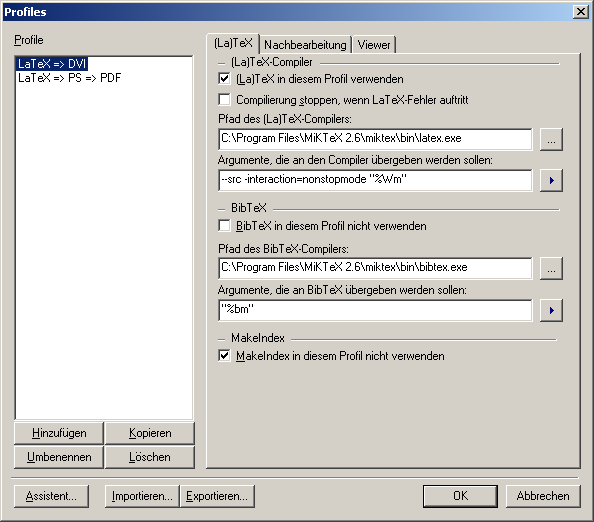
\includegraphics[width=0.49\textwidth]{techniccenter-profile-dvi-26} &
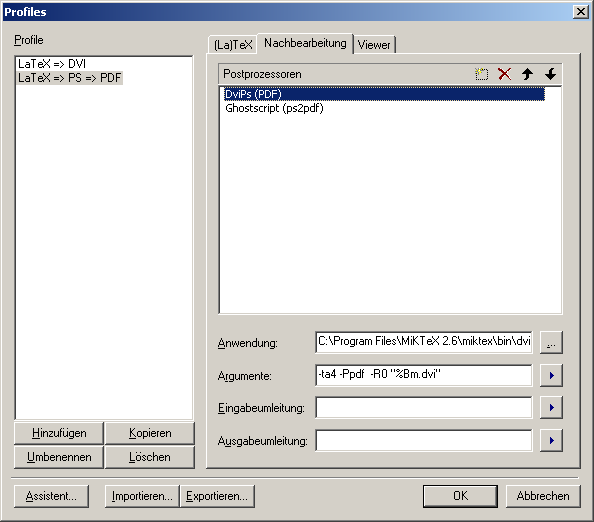
\includegraphics[width=0.49\textwidth]{techniccenter-profile-dvips-26} \\[4pt]
(a) & (b)
\end{tabular}
\caption{Spezifikation der Ausgabeprofile in TeXnicCenter.}
\label{fig:techniccenter-profile-latex}
\end{figure}

In der Datei \verb!tc_output_profiles_sumatra.tco! sind  folgende beiden "`maßgeschneiderten"' Ausgabeprofile für TexNicCenter angelegt (Import über \textsf{Build} $\rightarrow$ \textsf{Define Output Profiles ...}):
\begin{itemize}
	\item \verb!LaTeX => PDF (Sumatra)! -- Standard, direkte Erzeugung von PDF,
	\item \verb!LaTeX => PS => PDF (Sumatra)! -- PDF "`klassisch"' via DVI und PS.
\end{itemize}

\subsubsection{Profil "`\texttt{LaTeX => PDF (Sumatra)}"'}

Das ist das mit diesem Setup normalerweise verwendete Standardprofil.

\paragraph{(La)Tex:}
\begin{itemize}
  \item Path to the (La)TeX compiler: \\
        \begin{small} \verb!C:\Program Files (x86)\MiKTeX 2.9\miktex\bin\pdflatex.exe!\end{small}
  \item Command line arguments to pass to the compiler:\\
\begin{small}
   \verb!-synctex=-1 -interaction=nonstopmode "%pm"!
\end{small}
\end{itemize}

\paragraph{Postprocessor:} 
leer, kein Postprocessor notwendig.

\paragraph{Viewer:}
\begin{itemize}
\item Path of executable: \\
\begin{small}
    \verb!C:\Program Files (x86)\SumatraPDF\SumatraPDF.exe ! \\ 
    \verb!-inverse-search "\"C:\Program Files\TeXnicCenter\TEXCNTR.EXE\" !\\
    \verb!/ddecmd \"[goto('%f','%l')]\""!
\end{small}
%
\item View project's output: \\
\begin{small}
    \checkbox\ Command line argument \\\
    Command: \verb!"%bm.pdf"!
\end{small}
%
\item Forward search:\\
\begin{small}
    \checkbox\ DDE command \\\
    Command: \verb![ForwardSearch("%bm.pdf","%Wc",%l,0)]! \\
    Server: \verb!SUMATRA! \\
    Topic: \verb!Control!
\end{small}
\item Close document before running (La)TeX:\\
\begin{small}
    \checkbox\ Do not close
\end{small}
\end{itemize}


\subsubsection{Profil "`\texttt{LaTeX => PS => PDF (Sumatra)}"'}

Profil ausschließlich für den DVI-PS-Workflow (über DVI und PostScript).

\paragraph{(La)Tex:}
\begin{itemize}
  \item Path to the (La)TeX compiler: \\
        \begin{small} \verb!C:\Program Files (x86)\MiKTeX 2.9\miktex\bin\latex.exe!\end{small}
  \item Command line arguments to pass to the compiler:\\
\begin{small}
   \verb!-synctex=-1 -interaction=nonstopmode "%pm"!
\end{small}
\end{itemize}

\paragraph{Postprocessor:}
\begin{itemize}
  \item DviPS (PDF): \\
        \begin{small} 
        Executable: \verb!C:\Program Files (x86)\MiKTeX 2.9\miktex\bin\dvips.exe! \\
        Arguments: \verb!-ta4 -P pdf -R0 "%Bm.dvi"!
        \end{small}
  \item Ghostscript (ps2pdf):\\
  		\begin{small} 
        Executable: \verb!C:\Program Files (x86)\gs\gs9.04\bin\gswin32c.exe! \\
        Arguments: \verb!-q -dPDFSETTINGS=/prepress -sPAPERSIZE=a4 -dSAFER! \\
         \verb!-dBATCH -dNOPAUSE -sDEVICE=pdfwrite -sOutputFile="%bm.pdf"! \\
         \verb!-c save pop -f "%bm.ps"!
      \end{small}
\end{itemize}

\paragraph{Viewer:}
wie in Profil A. (\texttt{LaTeX => PDF (Sumatra)}).

\section{Tipps und offene Probleme:}

\begin{itemize}
\item \texttt{psfrag} funktioniert nicht mit \texttt{pdflatex} und es gibt auch leider keine Ersatzlösung. 
Wenn man \texttt{psfrag} braucht, dann muss man weiterhin über PostScript 
(\verb!LaTeX => PS => PDF!) arbeiten (was allerdings nunmehr auch mit \texttt{hyperref} kein Problem mehr ist).
%
\item Bei Verwendung des TexWorks-Editors (wird mit MikTeX ausgeliefert) sollte man die Standard-Zeichenkodierung von \emph{Unicode} (utf8) auf \emph{Latin-1} (ISO 8859-1) umstellen.
%
\item Adobe Illustrator kann beim Speichern als PDF die Bounding Box nicht setzen. 
Eine Möglichkeit ist, die Grafik zuerst als EPS zu exportieren und dann mit Acrobat in ein PDF zu konvertieren. 
%
\end{itemize}
\end{comment}



\begin{comment}
\section{Einstellungen für YAP (DVI-Viewer) im DVI-PS-Workflow}
\label{sec:YapEinstellung}

Im Standard-DVI-Viewer YAP lässt sich durch Mausklick auf das DVI-Dokument sehr leicht die zugehörige Stelle im Quelltext finden. Im Normalfall öffnet dann TeXnicCenter das zugehörige \latex-Dokument automatisch an der richtigen Stelle.
Das zugehörige "`Inverse DVI Search"' Kommando sollte sich bereits bei der Installation richtig einstellen.

Falls dies \emph{nicht} funktioniert, kann man in YAP diese Einstellung auch manuell über das Menü \textsf{View}\thinspace$\rightarrow$\thinspace\textsf{Options...} vornehmen, wie in Abb.\ \ref{fig:yap-inverse-search} gezeigt.
In diesem Fall lautet die vollständige Anweisung in "`Command Line"' folgendermaßen:
\begin{center}\footnotesize
\verb!"C:\Program Files (x86)\TeXnicCenter\TEXCNTR.EXE" /ddecmd "[goto('%f', '%l')]"!
\end{center}


\begin{figure}
\centering\small
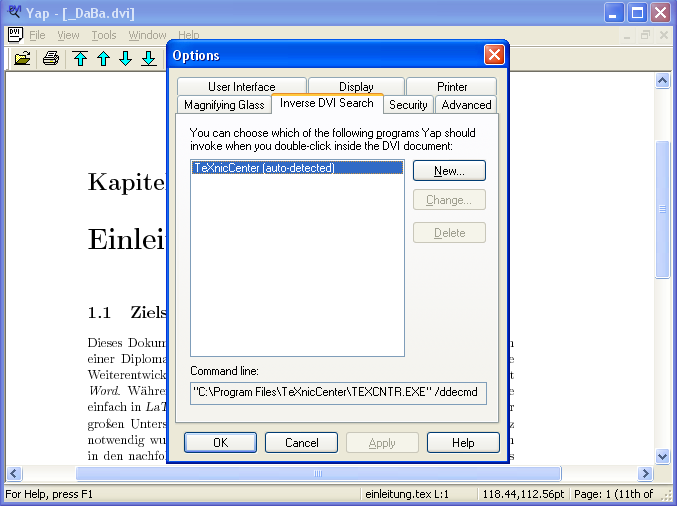
\includegraphics[width=1.0\textwidth]{yap-inverse-search-settings}
\caption{"`Inverse DVI Search"' Einstellung in YAP (über das Menü \textsf{View}\thinspace$\rightarrow$\thinspace\textsf{Options...}).}
\label{fig:yap-inverse-search}
\end{figure}

Latex
C:\Program Files\MiKTeX 2.6\miktex\bin\latex.exe
--src -interaction=nonstopmode "%Wm"

Bibtex
C:\Program Files\MiKTeX 2.6\miktex\bin\bibtex.exe
"%bm"

---

DviPs (PDF)
C:\Program Files\MiKTeX 2.6\miktex\bin\dvips.exe
-ta4 -Ppdf  -R0 "%Bm.dvi"

Ghostscript (ps2pdf)
C:\Program Files\gs\gs8.61\bin\gswin32c.exe
-sPAPERSIZE=a4 -dSAFER -dBATCH -dNOPAUSE -sDEVICE=pdfwrite -dPDFSETTINGS=/prepress -sOutputFile="%bm.pdf" -c save pop -f "%bm.ps"


YAP 
Options -> Inverse Search
"C:\Program Files\TeXnicCenter\TEXCNTR.EXE" /ddecmd "[goto('%f', '%l')]"

\end{comment}

	% Technische Ergänzungen


%%%----------------------------------------------------------
\MakeBibliography
%%%----------------------------------------------------------

%%%Messbox zur Druckkontrolle
\chapter*{Messbox zur Druckkontrolle}



\begin{center}
{\Large --- Druckgröße kontrollieren! ---}

\bigskip

\Messbox{100}{50} % Angabe der Breite/Hoehe in mm

\bigskip

{\Large --- Diese Seite nach dem Druck entfernen! ---}

\end{center}



\end{document}
